\chapter{Evaluation} % (10-15 pages)
\label{chap:eval}

\section{Data Gathering}
\noindent
Before evaluating the performance benchmarks, we need to understand the format of the benchmark output and how to parse the output into usable data.

\subsection*{Benchmark Output}

\begin{lstlisting}[language=prolog]
goos: linux
goarch: amd64
pkg: search
BenchmarkDepthFirstSearch/revisions=200,dataSize=100-16         	  393714	      8504 ns/op	    4249 B/op	      15 allocs/op
BenchmarkDepthFirstSearch/revisions=200,dataSize=1000-16        	  419702	      8537 ns/op	    4256 B/op	      15 allocs/op
BenchmarkDepthFirstSearch/revisions=2000,dataSize=100-16        	   39650	     90070 ns/op	   47976 B/op	      68 allocs/op
BenchmarkDepthFirstSearch/revisions=2000,dataSize=1000-16       	   39520	     92031 ns/op	   48012 B/op	      68 allocs/op
\end{lstlisting}
\medskip

The first items printed in the benchmark output are the two core \lstinline{Go} environment variables, \lstinline{GOOS} (Operating System, e.g., \lstinline{linux}) and \lstinline{GOARCH} (CPU Architecture, e.g., \lstinline{amd64}), followed by the \lstinline{pkg} (package name) which contains the benchmark functions being executed. Finally, the remaining lines contain the individual benchmark results, containing the following columns\cite{andile_2023}:

\begin{enumerate}
    \item \textless\lstinline{Name of benchmark}\textgreater\ -- \textless\lstinline{Number of CPU cores}\textgreater\\The name of the benchmark function being executed, followed by the number of CPU cores used to execute the benchmark. This is useful for identifying the number of CPU cores used to execute the benchmark, as the number of CPU cores used is not explicitly stated in the benchmark output.
    \item \textless\lstinline{Number of iterations}\textgreater\\The number of iterations executed by the benchmark function to produce the average performance metrics.
    \item \textless\lstinline{Average number of nanoseconds per operation}\textgreater\\The average number of nanoseconds taken to execute a single operation of the benchmark function.
    \item \textless\lstinline{Average number of Bytes allocated per operation}\textgreater\\The average number of Bytes allocated to execute a single operation of the benchmark function.
    \item \textless\lstinline{Average number of memory allocations per operation}\textgreater\\The average number of memory allocations to execute a single operation of the benchmark function.
\end{enumerate}

\subsection*{Data Parsing}
A \lstinline{Python} script was employed to parse usable data from the \lstinline{Go} benchmark logs. The script leveraged regular expressions to identify and extract key performance metrics such as the number of iterations, time taken per operation (in nanoseconds), memory allocated per operation (in bytes), and the number of memory allocations per operation. This information was then stored in a CSV file format, facilitating easy data analysis and visualisation.

\begin{lstlisting}[language=python]
import csv
import re

benchmark_pattern = re.compile(
    r"Benchmark([\w_]+)/revisions=(\d+),dataSize=(\d+)-(\d+)
        \s+(\d+)\s+(\d+) ns/op\s+(\d+) B/op\s+(\d+) allocs/op"
)

csv_headers = [
    "benchmark_name",
    "num_revisions",
    "data_size",
    "num_cpus",
    "iterations",
    "ns_per_op",
    "bytes_per_op",
    "allocs_per_op",
]

for log_file, csv_file in log_files.items():
    with open(log_file, "r") as f:
        content = f.read()

    benchmarks = benchmark_pattern.findall(content)
    
    with open(csv_file, "w", newline="") as f:
        writer = csv.writer(f)
        writer.writerow(csv_headers)
        for benchmark in benchmarks:
            writer.writerow(benchmark)

\end{lstlisting}

\subsection*{Performance Metrics}
In order to compare the performance of the implemented algorithms and data structures, we considered the following key performance metrics:

\paragraph{Execution time \(ns\_per\_op\)}
The time taken per operation (in nanoseconds) was a primary factor in determining the efficiency of the algorithms. Lower execution times indicate better performance.

\paragraph{Memory usage \(bytes\_per\_op\)}
Memory allocated per operation (in bytes) was another crucial aspect to evaluate, as efficient algorithms should minimise memory consumption.

\paragraph{Memory allocations \(allocs\_per\_op\)}
The number of memory allocations per operation was also taken into account, as fewer allocations generally indicate a more optimised algorithm.

\section{Data Structures}

\subsection{Doubly Linked List}

\begin{table}[h]
    \centering
    \begin{tabular}{|r|r|r|r|r|}
        \hline
        \multicolumn{1}{|c|}{\textbf{num\_revisions}} & \multicolumn{1}{c|}{\textbf{data\_size}} & \multicolumn{1}{c|}{\textbf{ns\_per\_op}} & \multicolumn{1}{c|}{\textbf{bytes\_per\_op}} & \multicolumn{1}{c|}{\textbf{allocs\_per\_op}} \\ \hline
        200 Revs                                      & 100 byte/rev                             & 714030                                    & 35200                                        & 600                                           \\ \hline
        200 Revs                                      & 1000 byte/rev                            & 3989548                                   & 217604                                       & 600                                           \\ \hline
        200 Revs                                      & 10000 byte/rev                           & 36909724                                  & 2060860                                      & 600                                           \\ \hline
        2000 Revs                                     & 100 byte/rev                             & 10124801                                  & 352003                                       & 6000                                          \\ \hline
        2000 Revs                                     & 1000 byte/rev                            & 40641532                                  & 2176026                                      & 6000                                          \\ \hline
        2000 Revs                                     & 10000 byte/rev                           & 344262304                                 & 20608074                                     & 6000                                          \\ \hline
        20000 Revs                                    & 100 byte/rev                             & 455200208                                 & 3520027                                      & 60000                                         \\ \hline
        20000 Revs                                    & 1000 byte/rev                            & 759428984                                 & 21760746                                     & 60003                                         \\ \hline
        20000 Revs                                    & 10000 byte/rev                           & 3792506585                                & 206080096                                    & 60001                                         \\ \hline
    \end{tabular}
    \caption{Performance metrics for the Doubly Linked List implementation.}
    \label{tab:doubly-linked-list-benchmark-results}
\end{table}

\begin{figure}[H]
    \centering
    \begin{subfigure}[b]{0.8\textwidth}
        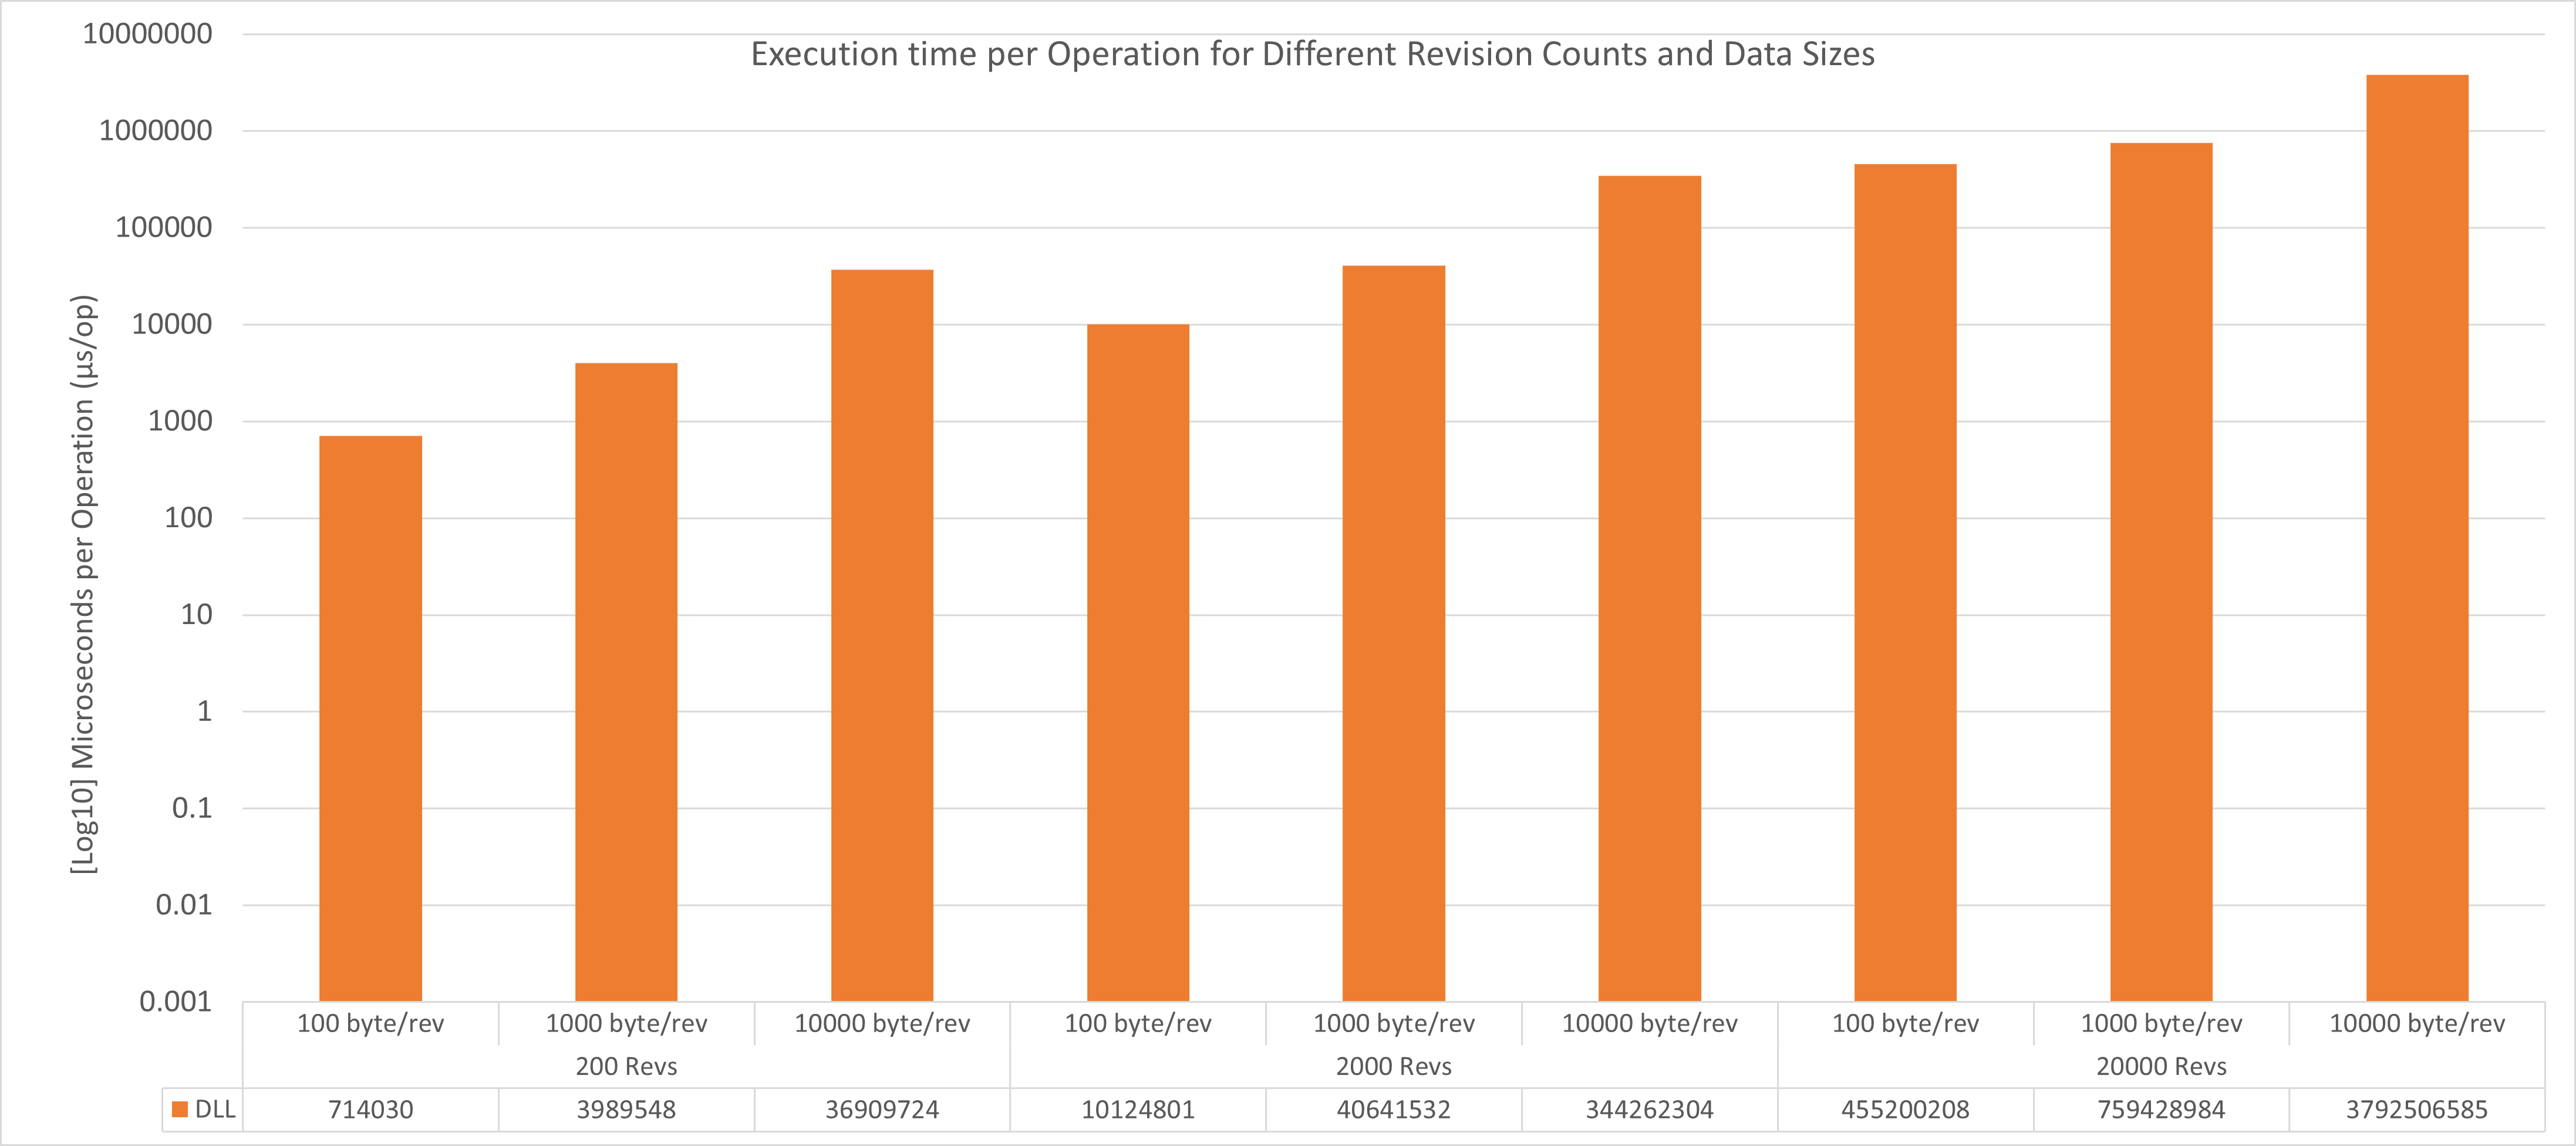
\includegraphics[width=1\linewidth]{charts/dll_ns_all.png}
        \caption{Execution Time}
        \label{fig:doubly-linked-list-execution-time}
    \end{subfigure}

    \begin{subfigure}[b]{0.8\textwidth}
        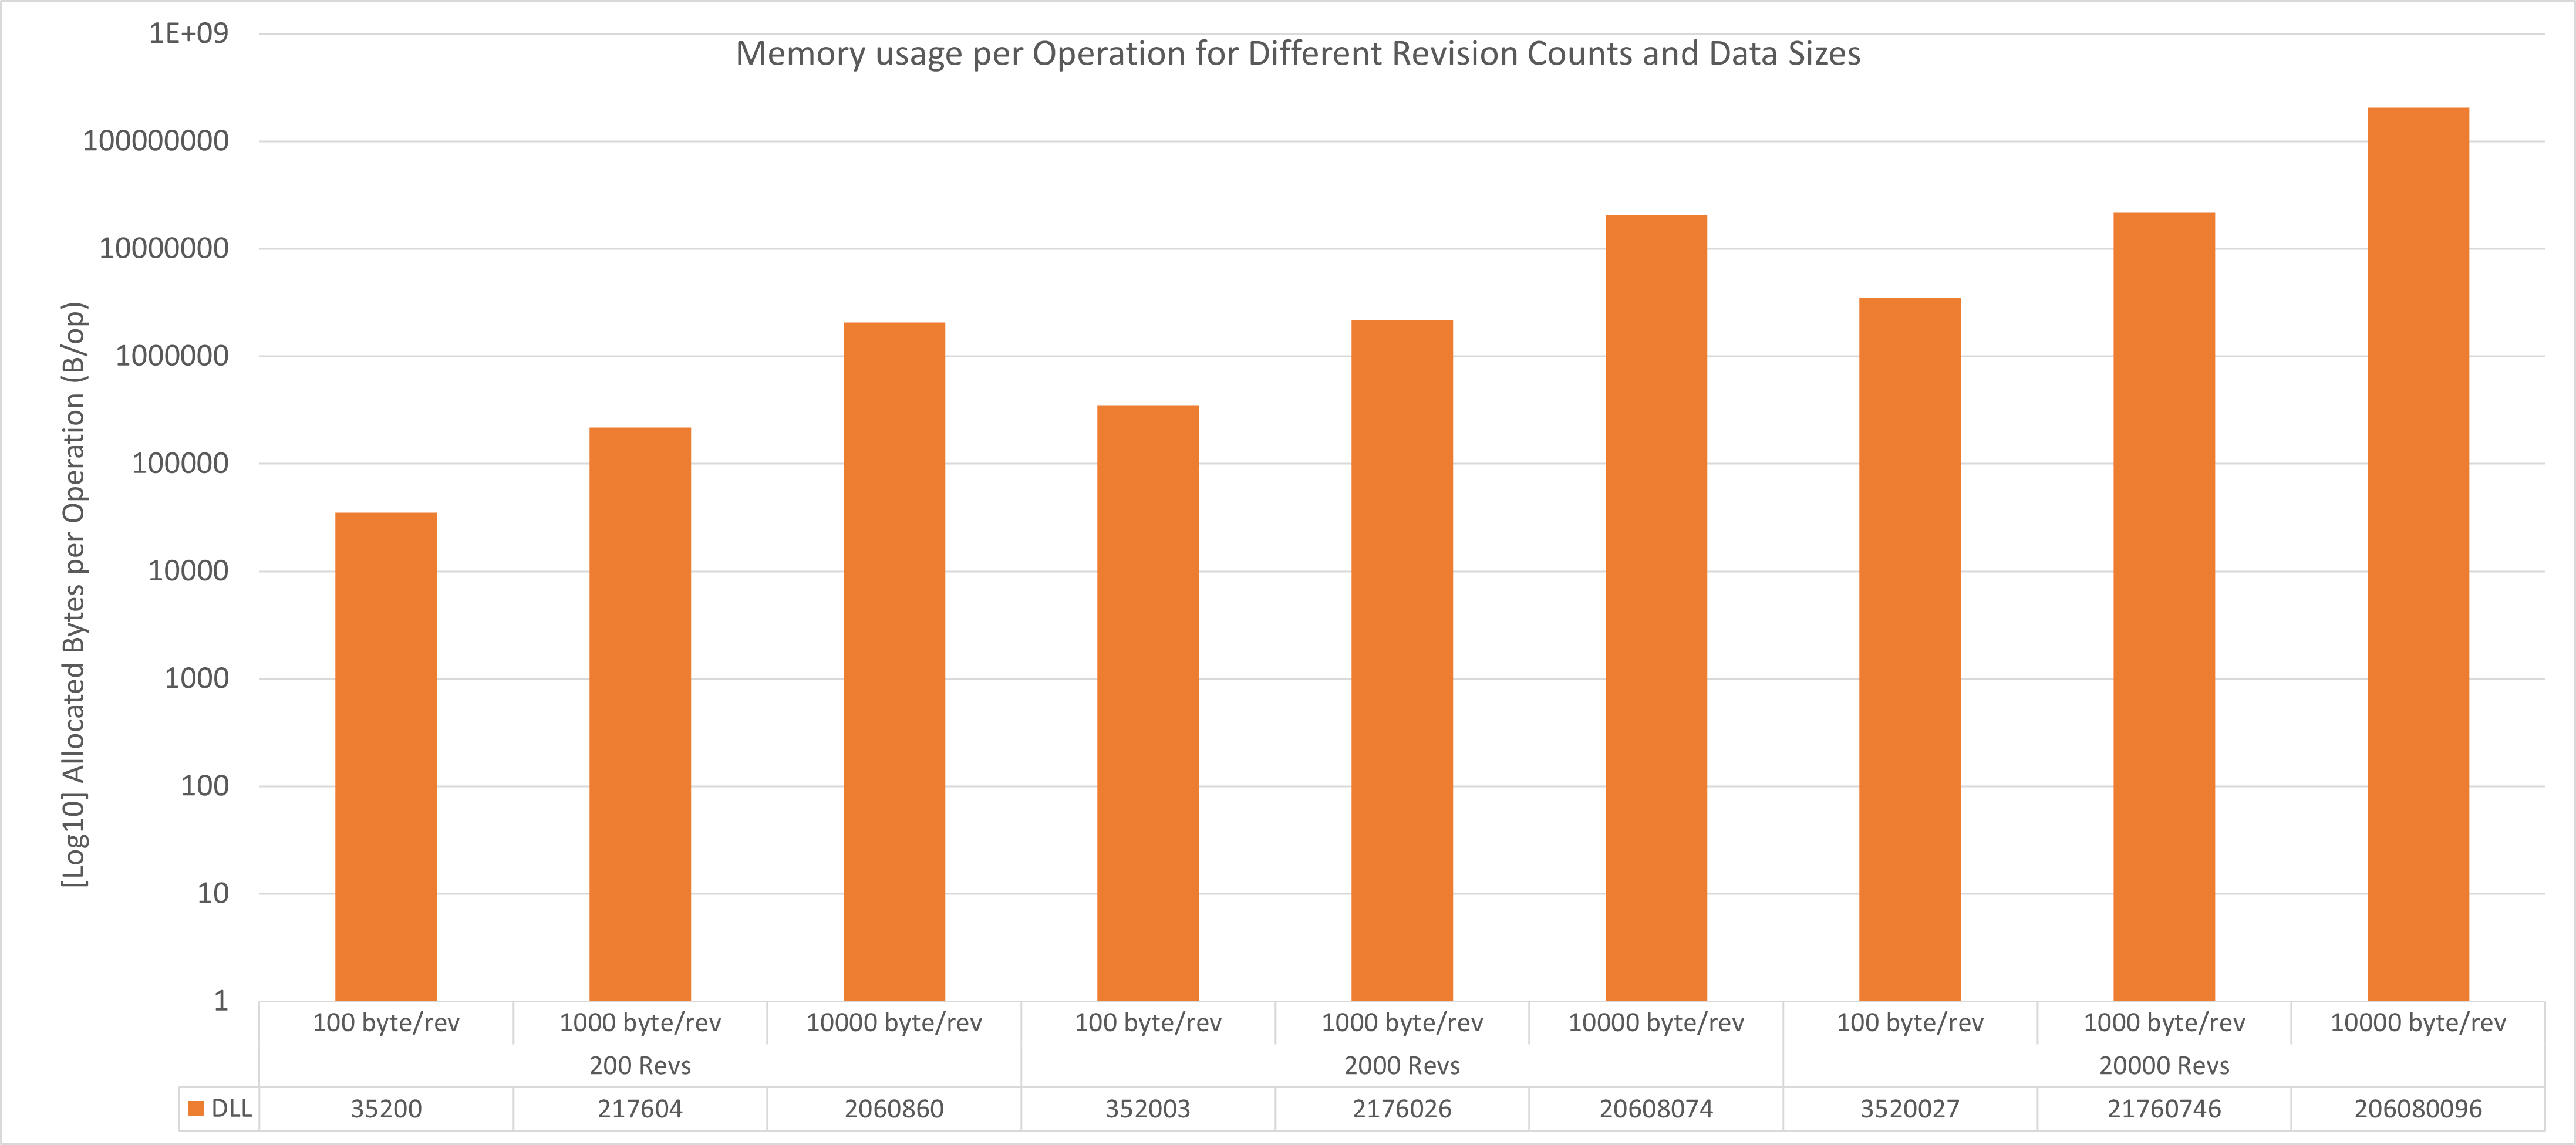
\includegraphics[width=1\linewidth]{charts/dll_bytes_all.png}
        \caption{Memory Usage}
        \label{fig:doubly-linked-list-memory-usage}
    \end{subfigure}

    \begin{subfigure}[b]{0.8\textwidth}
        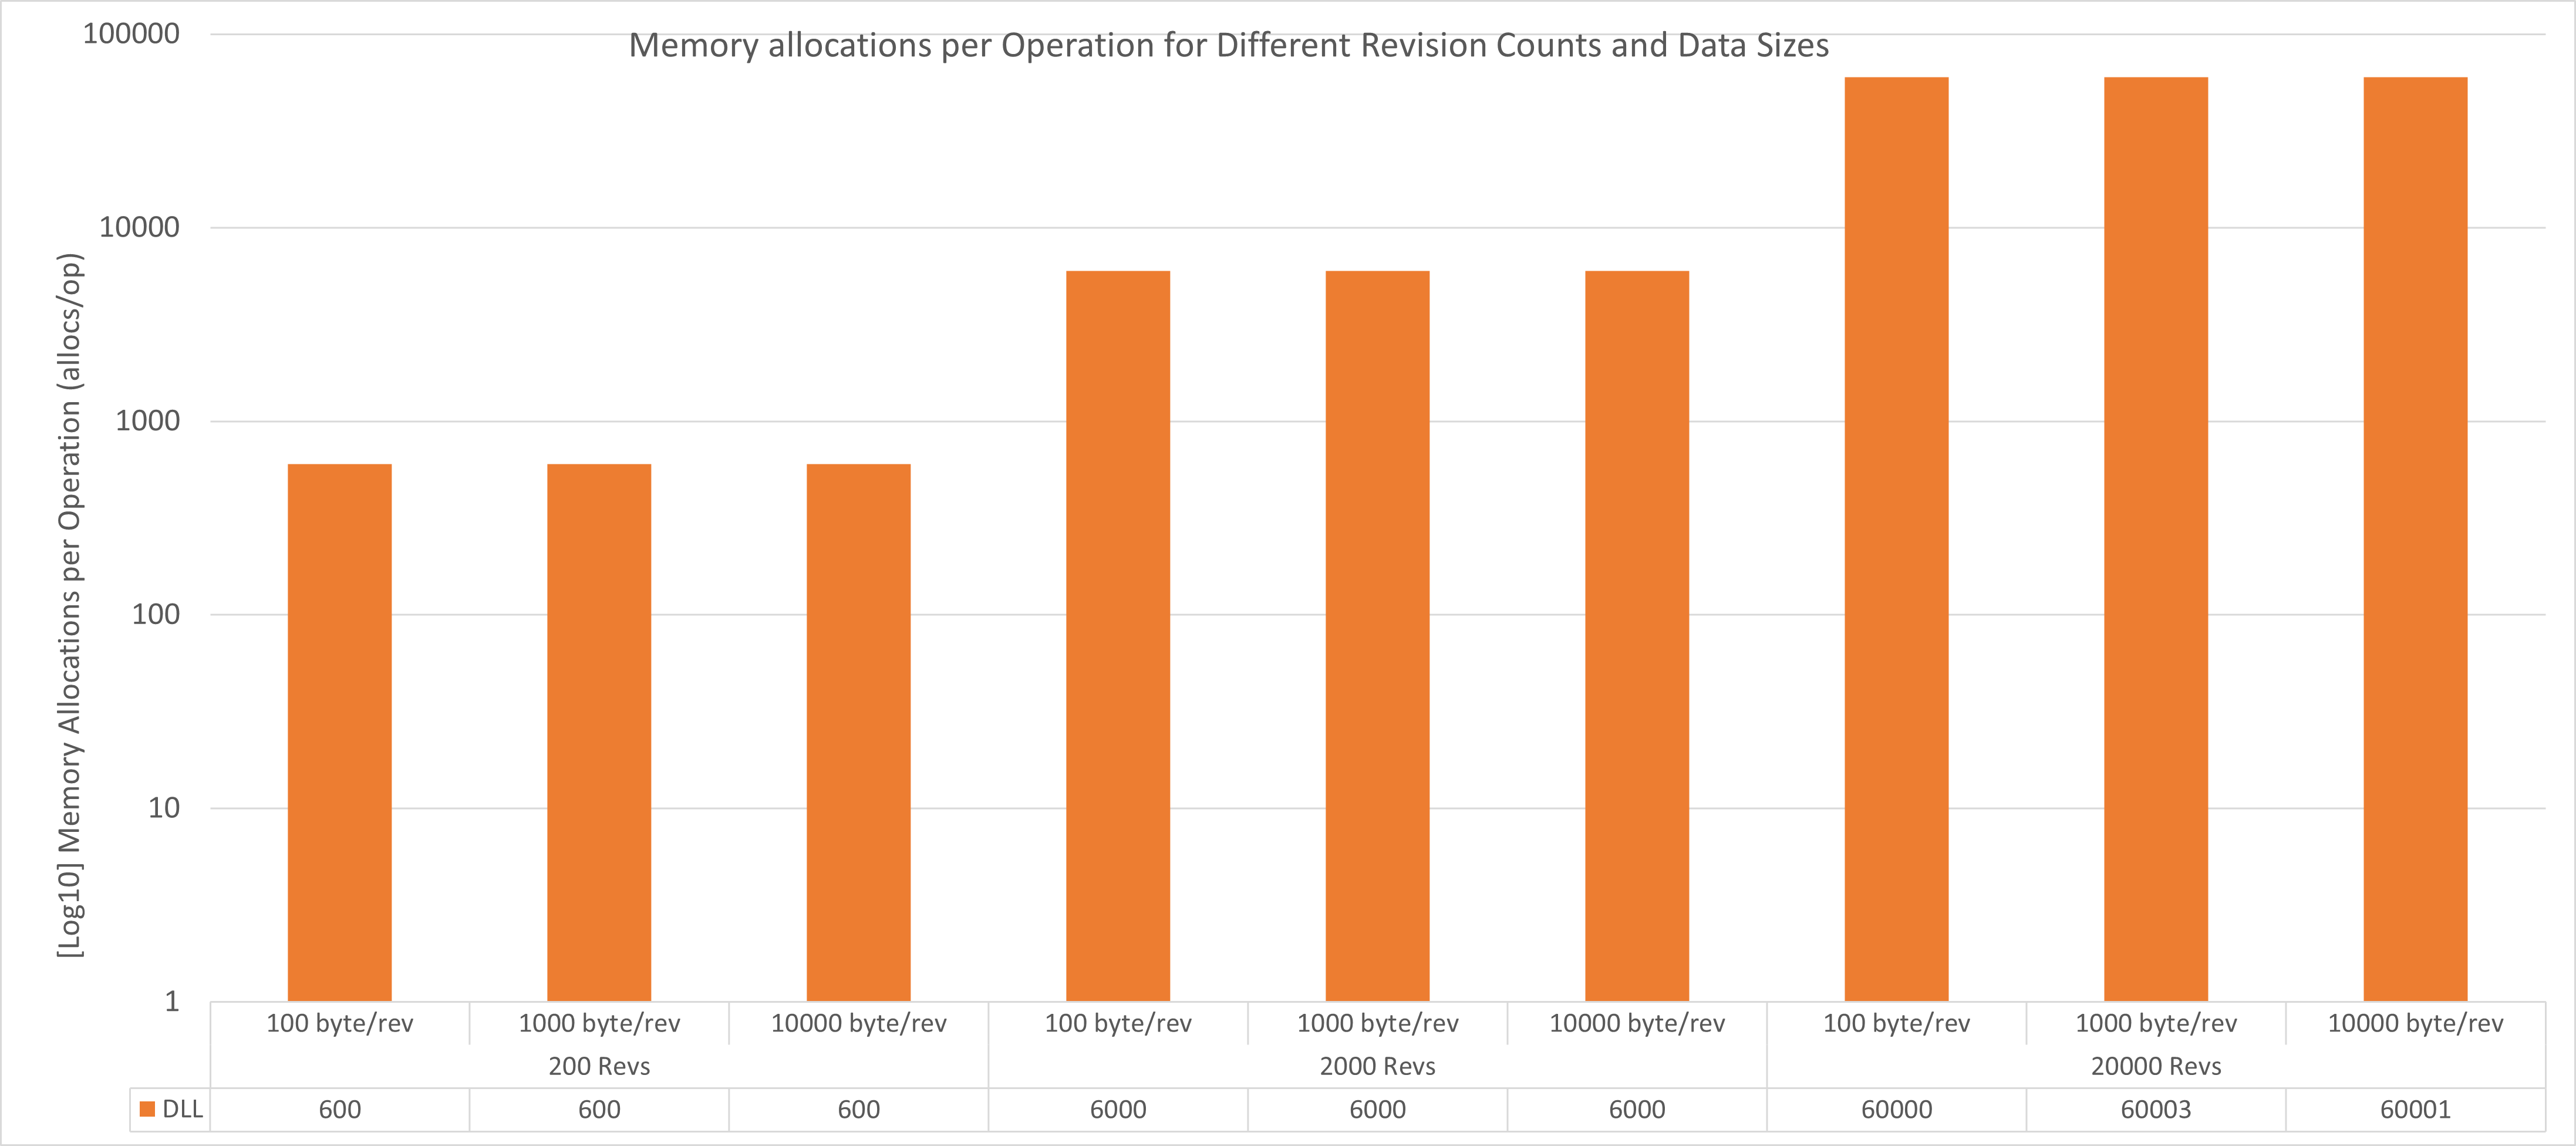
\includegraphics[width=1\linewidth]{charts/dll_allocs_all.png}
        \caption{Memory Allocations}
        \label{fig:doubly-linked-list-memory-allocations}
    \end{subfigure}

    \caption{Performance metrics for the Doubly Linked List implementation.}
    \label{fig:doubly-linked-list-performance-metrics}
\end{figure}

\subsection{Binary Search Tree}

\begin{table}[h]
    \centering
    \begin{tabular}{|r|r|r|r|r|}
        \hline
        \multicolumn{1}{|c|}{\textbf{num\_revisions}} & \multicolumn{1}{c|}{\textbf{data\_size}} & \multicolumn{1}{c|}{\textbf{ns\_per\_op}} & \multicolumn{1}{c|}{\textbf{bytes\_per\_op}} & \multicolumn{1}{c|}{\textbf{allocs\_per\_op}} \\ \hline
        200 Revs                                      & 100 byte/rev                             & 799807                                    & 35169                                        & 599                                           \\ \hline
        200 Revs                                      & 1000 byte/rev                            & 3748116                                   & 217569                                       & 599                                           \\ \hline
        200 Revs                                      & 10000 byte/rev                           & 34207201                                  & 2060844                                      & 599                                           \\ \hline
        2000 Revs                                     & 100 byte/rev                             & 13248417                                  & 351969                                       & 5999                                          \\ \hline
        2000 Revs                                     & 1000 byte/rev                            & 43291630                                  & 2176004                                      & 5999                                          \\ \hline
        2000 Revs                                     & 10000 byte/rev                           & 345554877                                 & 20608021                                     & 5999                                          \\ \hline
        20000 Revs                                    & 100 byte/rev                             & 754987022                                 & 3520006                                      & 59999                                         \\ \hline
        20000 Revs                                    & 1000 byte/rev                            & 1033066809                                & 21760032                                     & 59999                                         \\ \hline
        20000 Revs                                    & 10000 byte/rev                           & 4043692919                                & 206080256                                    & 60002                                         \\ \hline
    \end{tabular}
    \caption{Performance metrics for the Binary Search Tree implementation.}
    \label{tab:binary-search-tree-benchmark-results}
\end{table}

\begin{figure}[H]
    \centering
    \begin{subfigure}[b]{0.8\textwidth}
        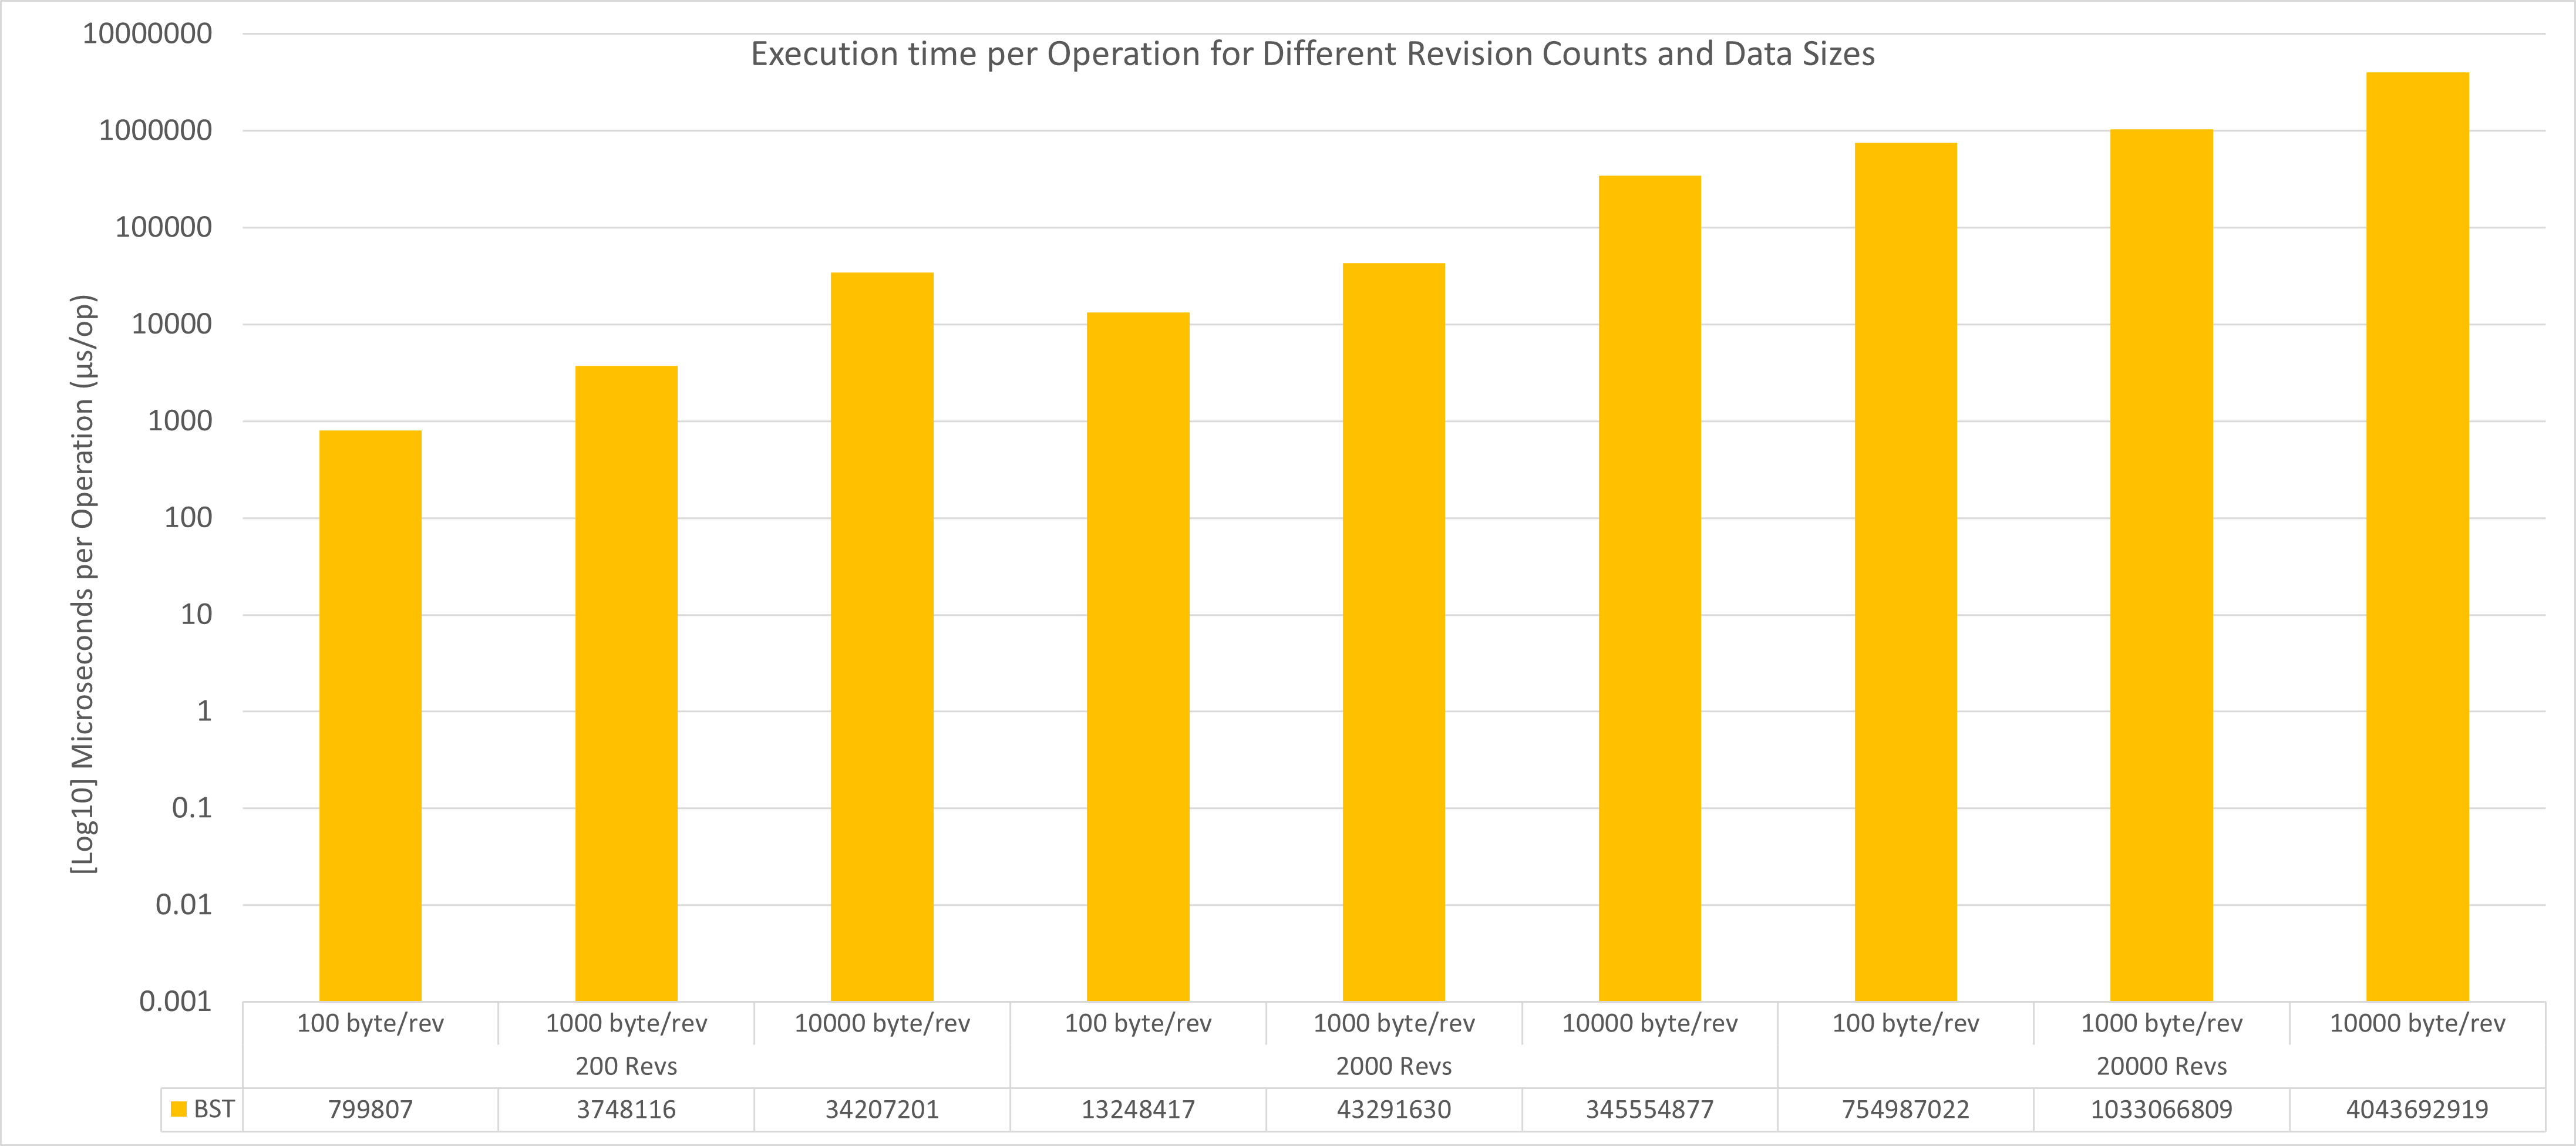
\includegraphics[width=1\linewidth]{charts/bst_ns_all.png}
        \caption{Execution Time}
        \label{fig:binary-search-tree-execution-time}
    \end{subfigure}

    \begin{subfigure}[b]{0.8\textwidth}
        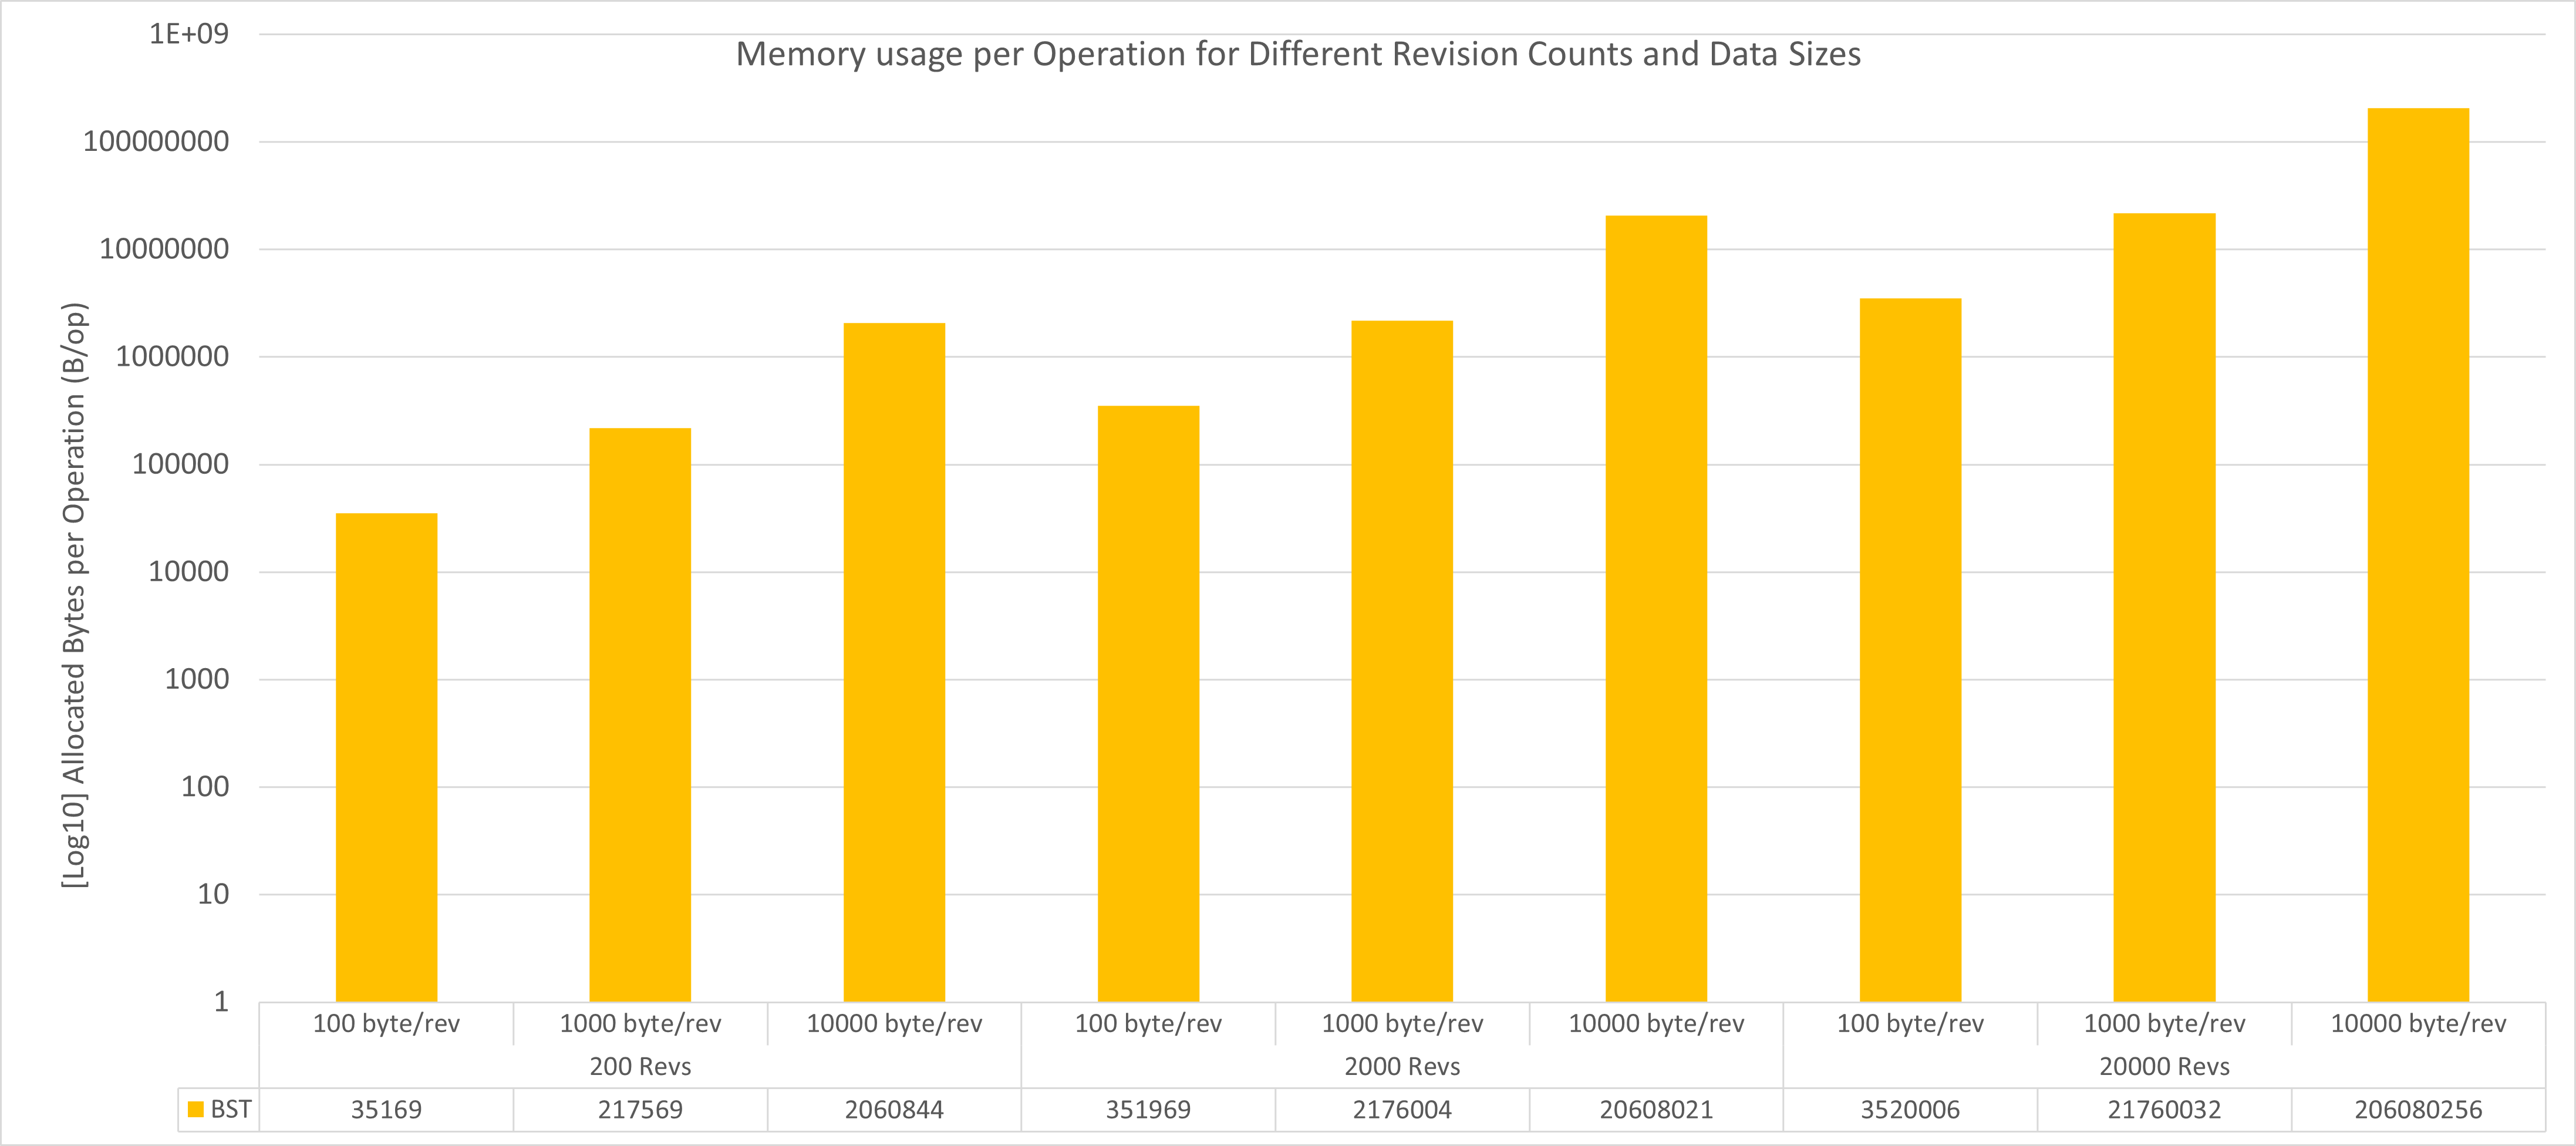
\includegraphics[width=1\linewidth]{charts/bst_bytes_all.png}
        \caption{Memory Usage}
        \label{fig:binary-search-tree-memory-usage}
    \end{subfigure}

    \begin{subfigure}[b]{0.8\textwidth}
        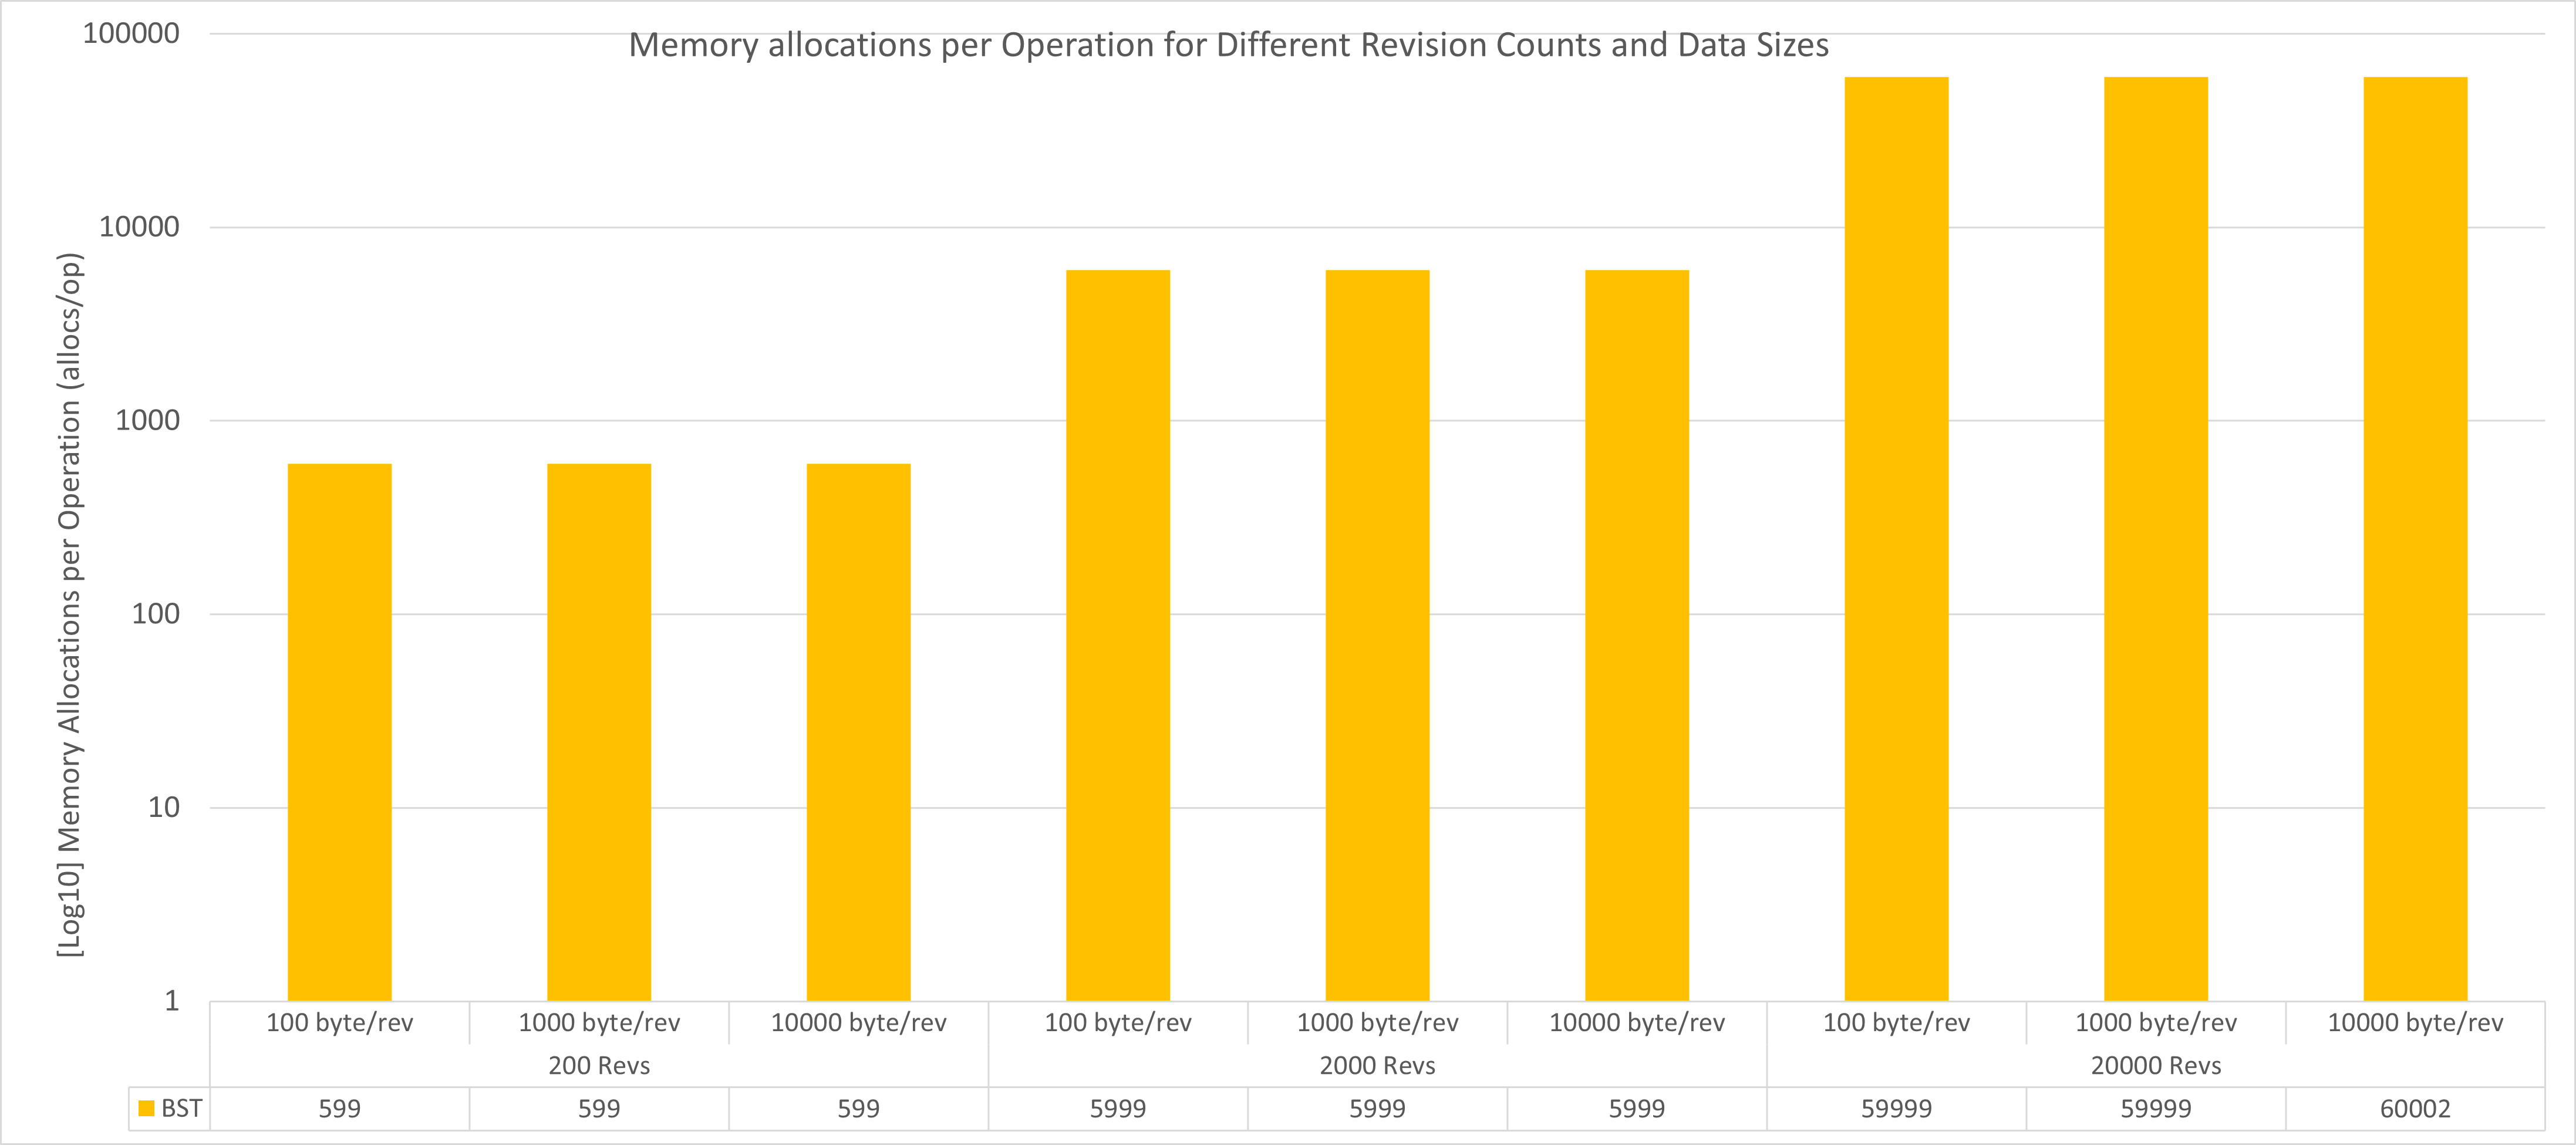
\includegraphics[width=1\linewidth]{charts/bst_allocs_all.png}
        \caption{Memory Allocations}
        \label{fig:binary-search-tree-memory-allocations}
    \end{subfigure}

    \caption{Performance metrics for the Binary Search Tree implementation.}
    \label{fig:binary-search-tree-performance-metrics}
\end{figure}

\subsection{Directed Acyclic Graph}

\begin{table}[h]
    \centering
    \begin{tabular}{|r|r|r|r|r|}
        \hline
        \multicolumn{1}{|c|}{\textbf{num\_revisions}} & \multicolumn{1}{c|}{\textbf{data\_size}} & \multicolumn{1}{c|}{\textbf{ns\_per\_op}} & \multicolumn{1}{c|}{\textbf{bytes\_per\_op}} & \multicolumn{1}{c|}{\textbf{allocs\_per\_op}} \\ \hline
        200 Revs                                      & 100 byte/rev                             & 727843                                    & 55593                                        & 1008                                          \\ \hline
        200 Revs                                      & 1000 byte/rev                            & 3734667                                   & 237970                                       & 1008                                          \\ \hline
        200 Revs                                      & 10000 byte/rev                           & 34303289                                  & 2081246                                      & 1009                                          \\ \hline
        2000 Revs                                     & 100 byte/rev                             & 7260065                                   & 618806                                       & 10057                                         \\ \hline
        2000 Revs                                     & 1000 byte/rev                            & 37559841                                  & 2442897                                      & 10058                                         \\ \hline
        2000 Revs                                     & 10000 byte/rev                           & 343197450                                 & 20875066                                     & 10057                                         \\ \hline
        20000 Revs                                    & 100 byte/rev                             & 73485424                                  & 5824547                                      & 100473                                        \\ \hline
        20000 Revs                                    & 1000 byte/rev                            & 374157517                                 & 24065936                                     & 100484                                        \\ \hline
        20000 Revs                                    & 10000 byte/rev                           & 3492010230                                & 208384192                                    & 100473                                        \\ \hline
    \end{tabular}
    \caption{Performance metrics for the Directed Acyclic Graph implementation.}
    \label{tab:directed-acyclic-graph-benchmark-results}
\end{table}

\begin{figure}[H]
    \centering
    \begin{subfigure}[b]{0.8\textwidth}
        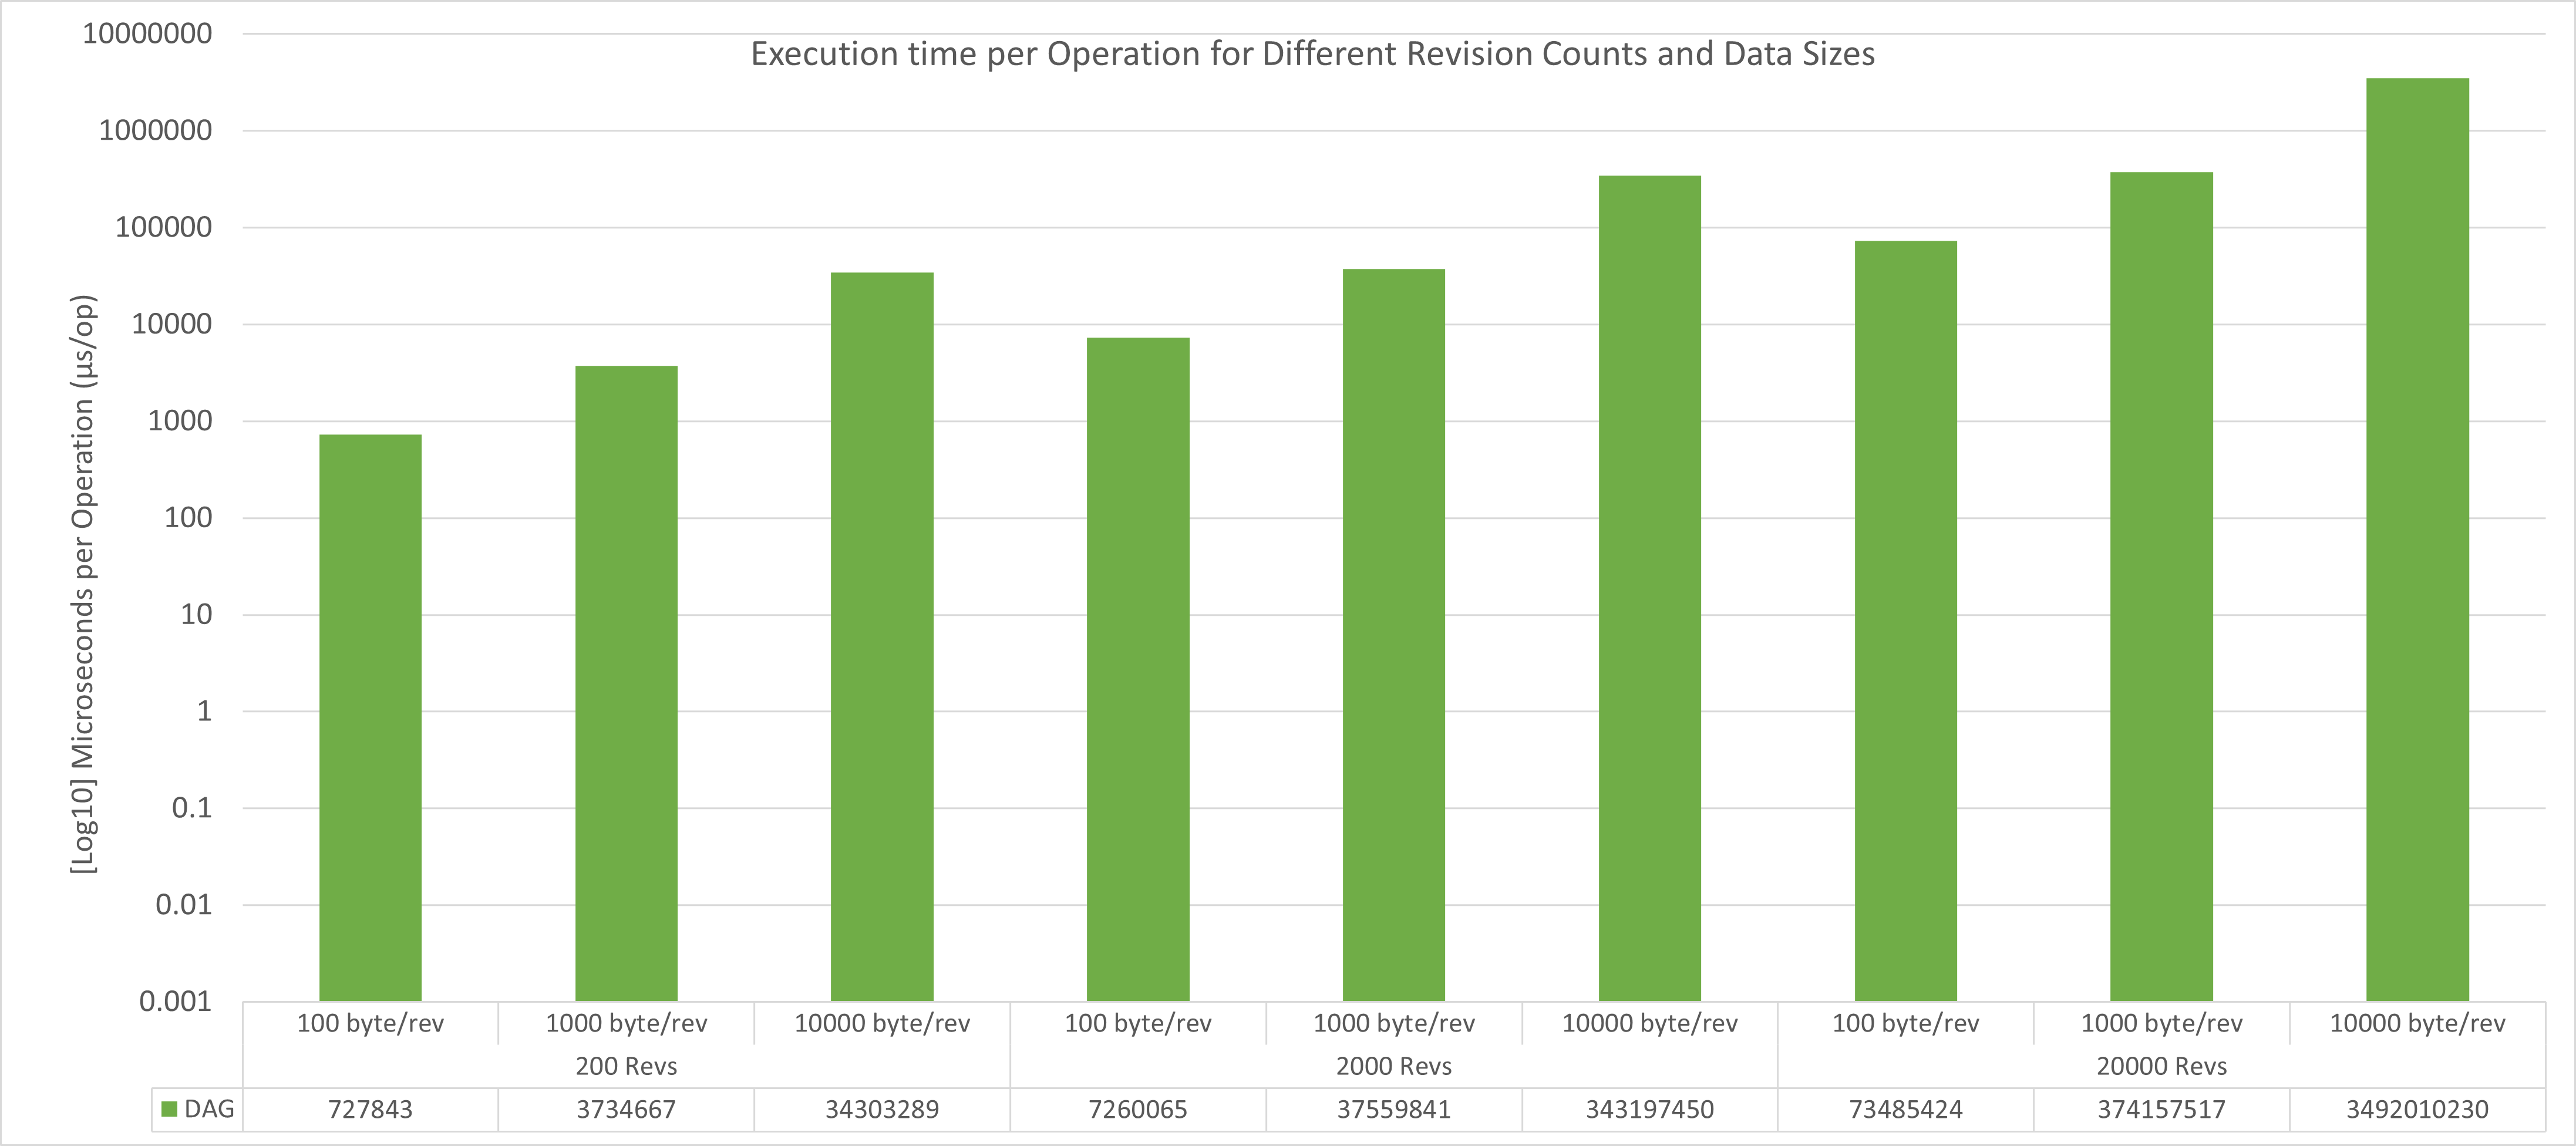
\includegraphics[width=1\linewidth]{charts/dag_ns_all.png}
        \caption{Execution Time}
        \label{fig:directed-acyclic-graph-execution-time}
    \end{subfigure}

    \begin{subfigure}[b]{0.8\textwidth}
        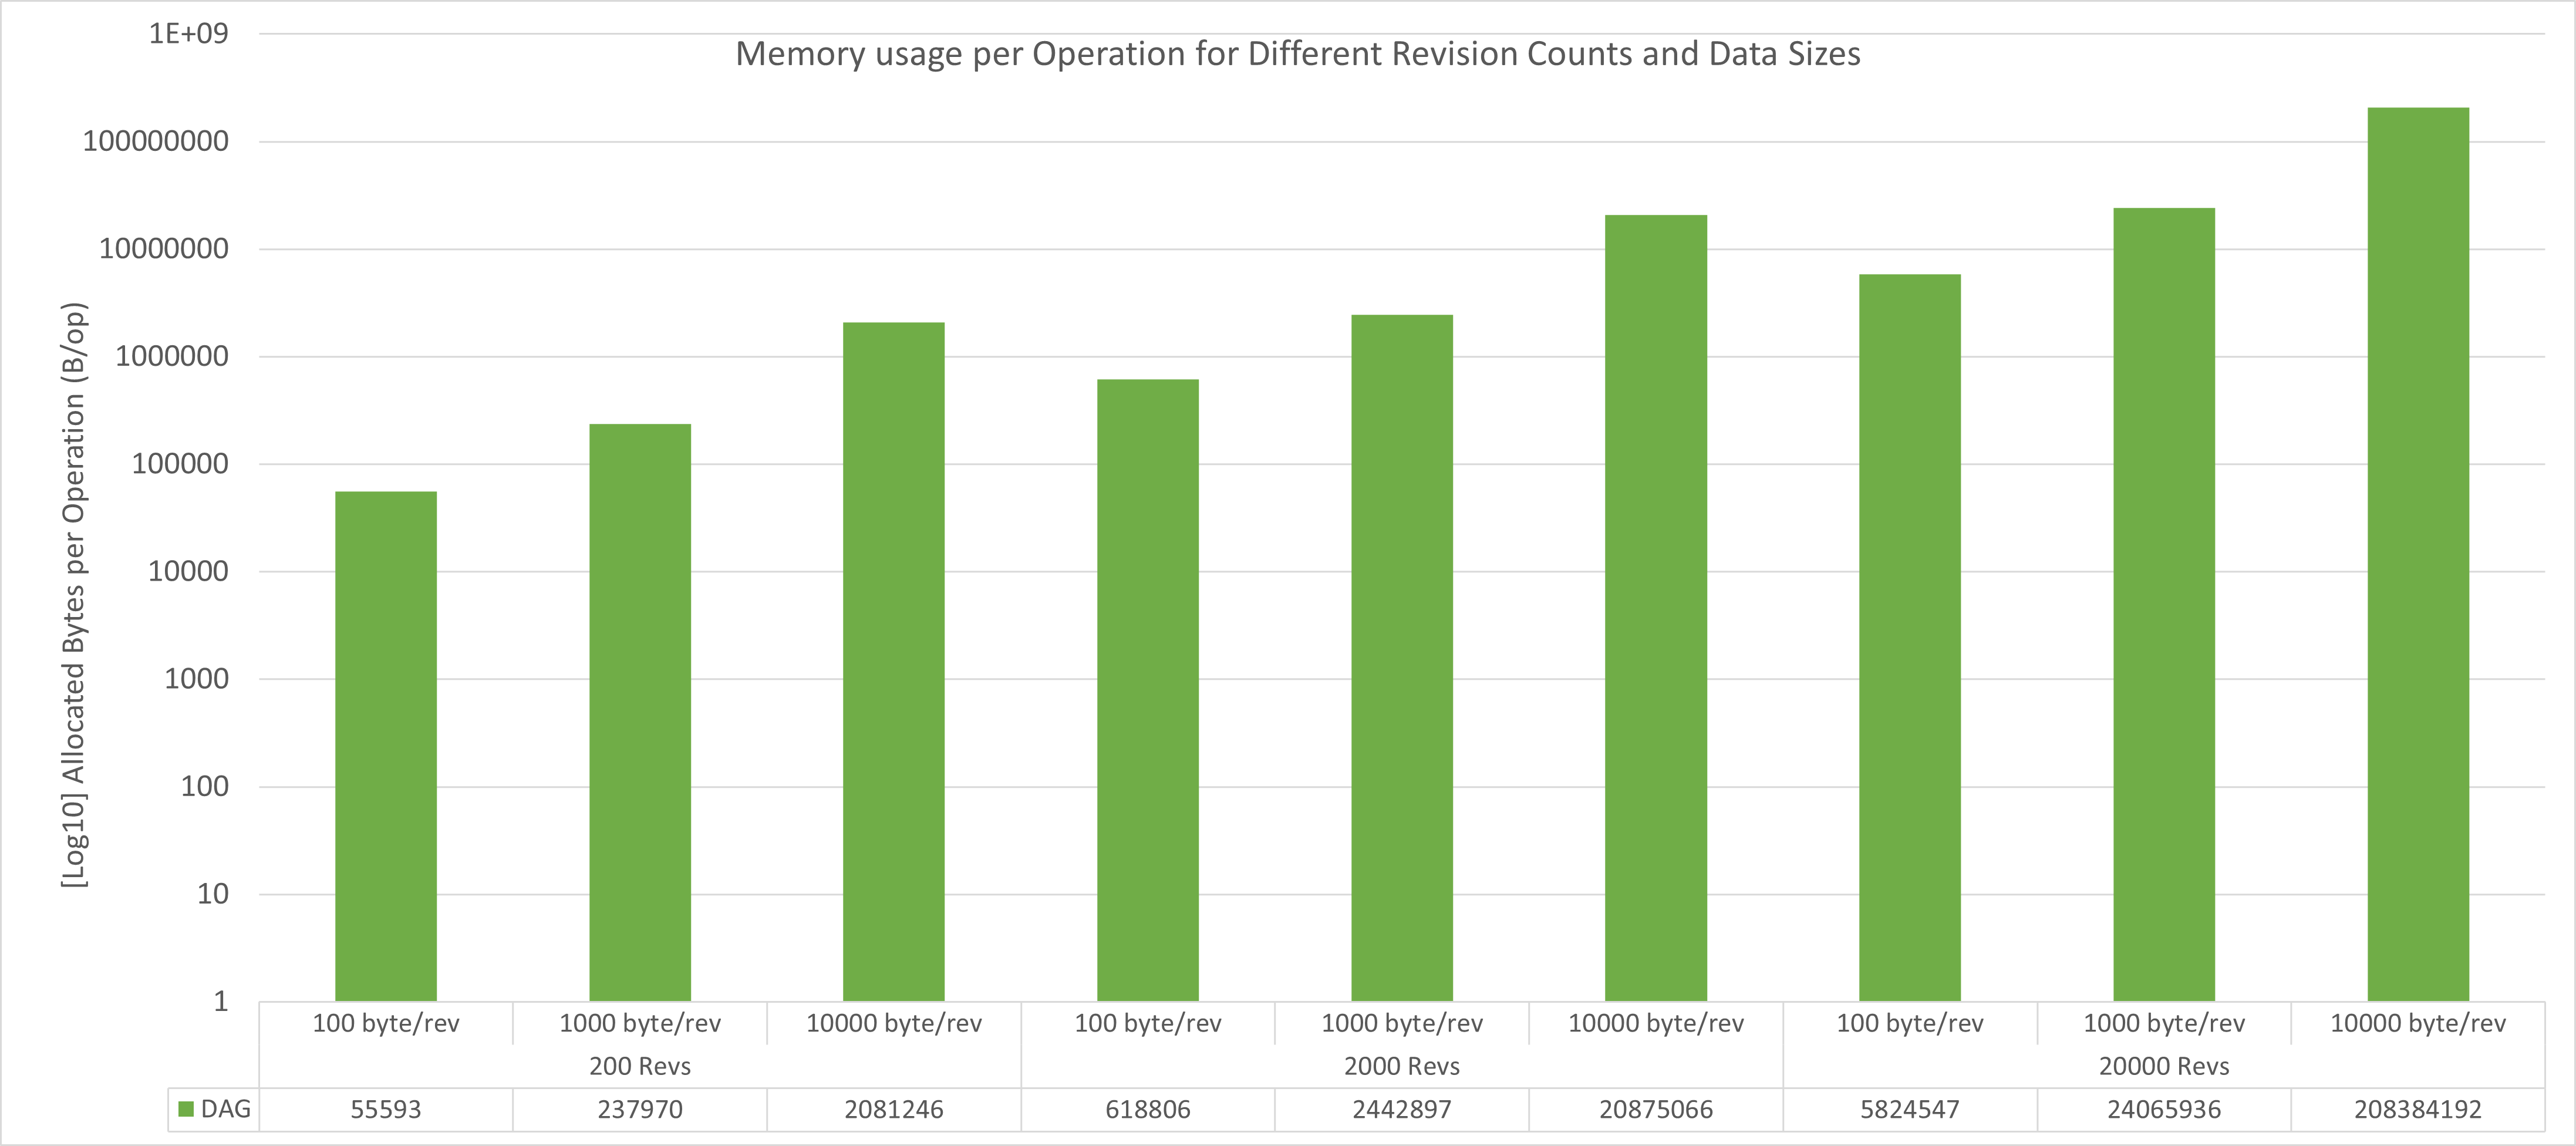
\includegraphics[width=1\linewidth]{charts/dag_bytes_all.png}
        \caption{Memory Usage}
        \label{fig:directed-acyclic-graph-memory-usage}
    \end{subfigure}

    \begin{subfigure}[b]{0.8\textwidth}
        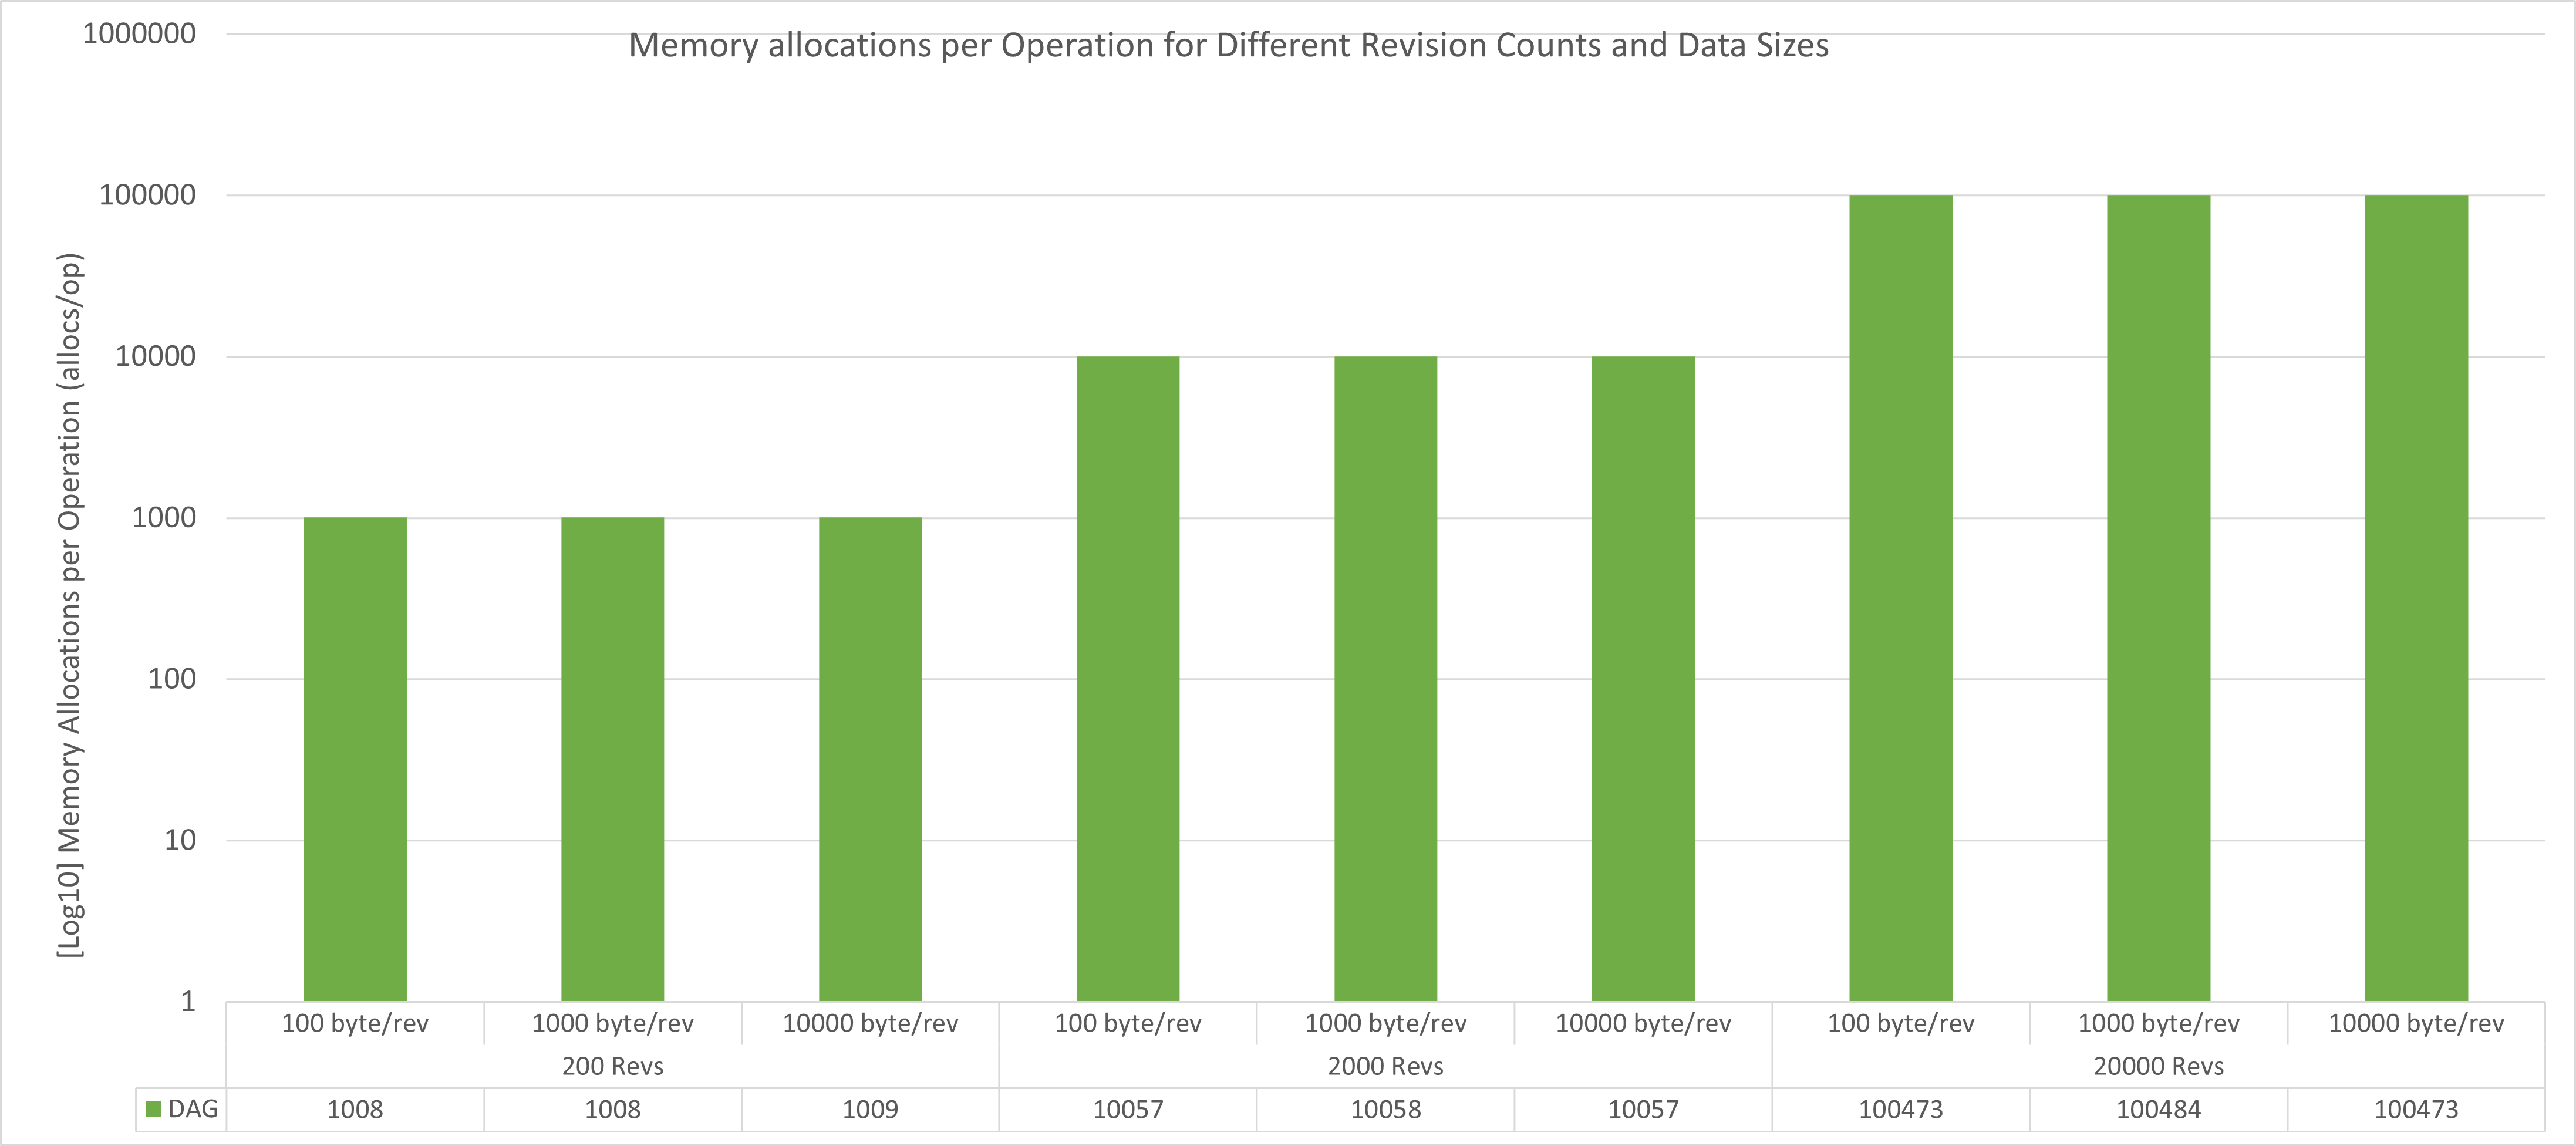
\includegraphics[width=1\linewidth]{charts/dag_allocs_all.png}
        \caption{Memory Allocations}
        \label{fig:directed-acyclic-graph-memory-allocations}
    \end{subfigure}

    \caption{Performance metrics for the Directed Acyclic Graph implementation.}
    \label{fig:directed-acyclic-graph-performance-metrics}
\end{figure}

\subsection{Comparison}

\begin{figure}[H]
    \centering
    \begin{subfigure}[b]{0.75\textwidth}
        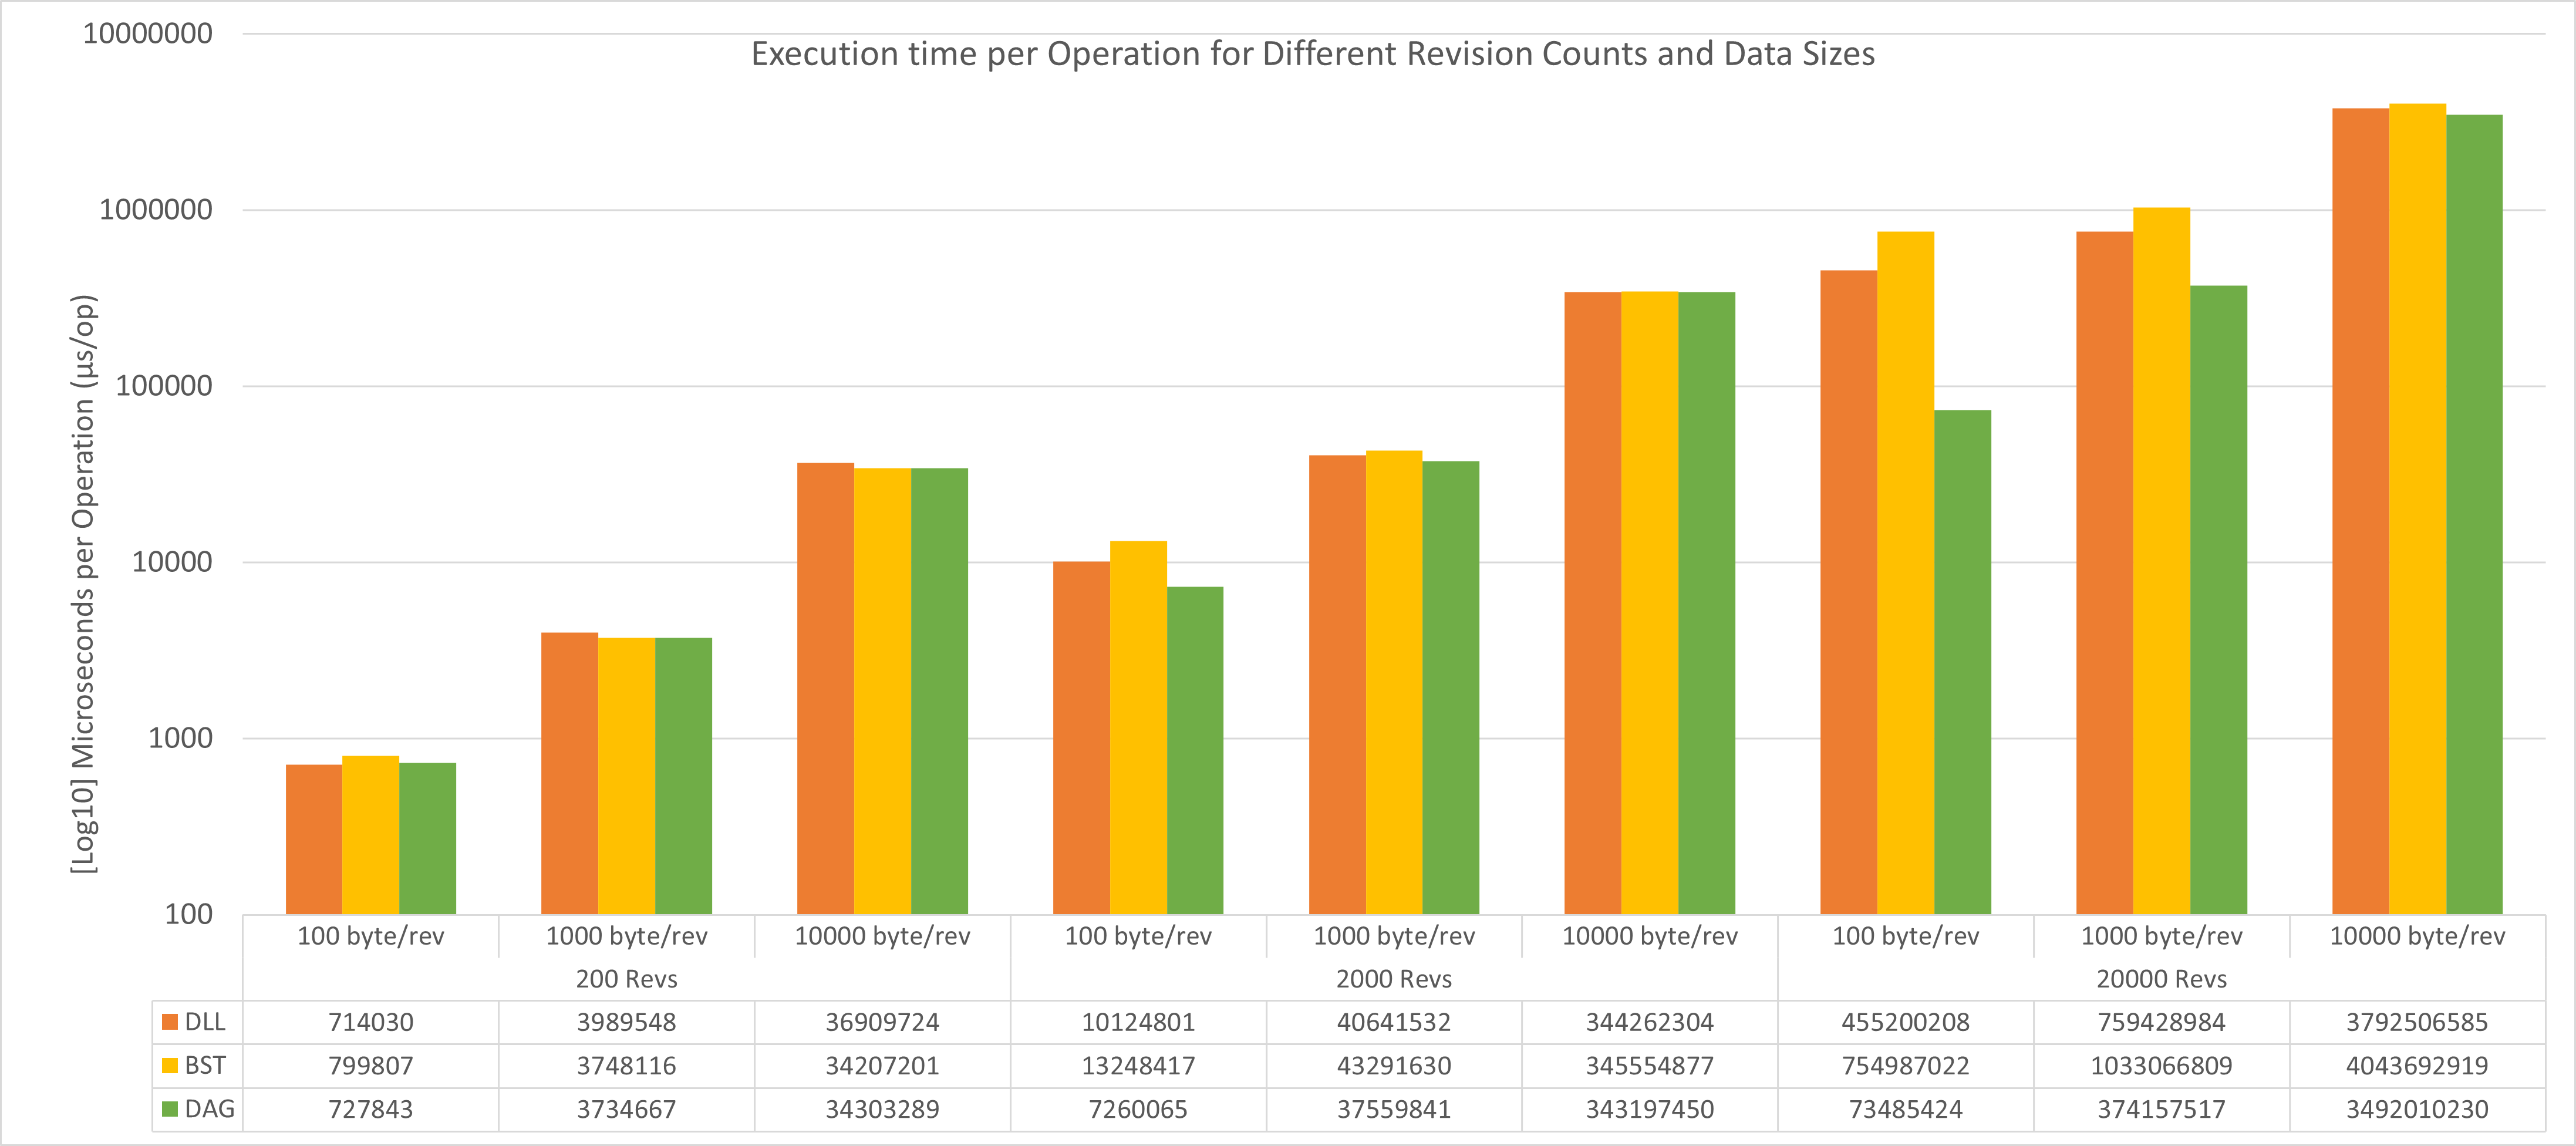
\includegraphics[width=1\linewidth]{charts/dataStruct_ns_all.png}
        \caption{Execution Time}
        \label{fig:data-structure-execution-time}
    \end{subfigure}

    \begin{subfigure}[b]{0.75\textwidth}
        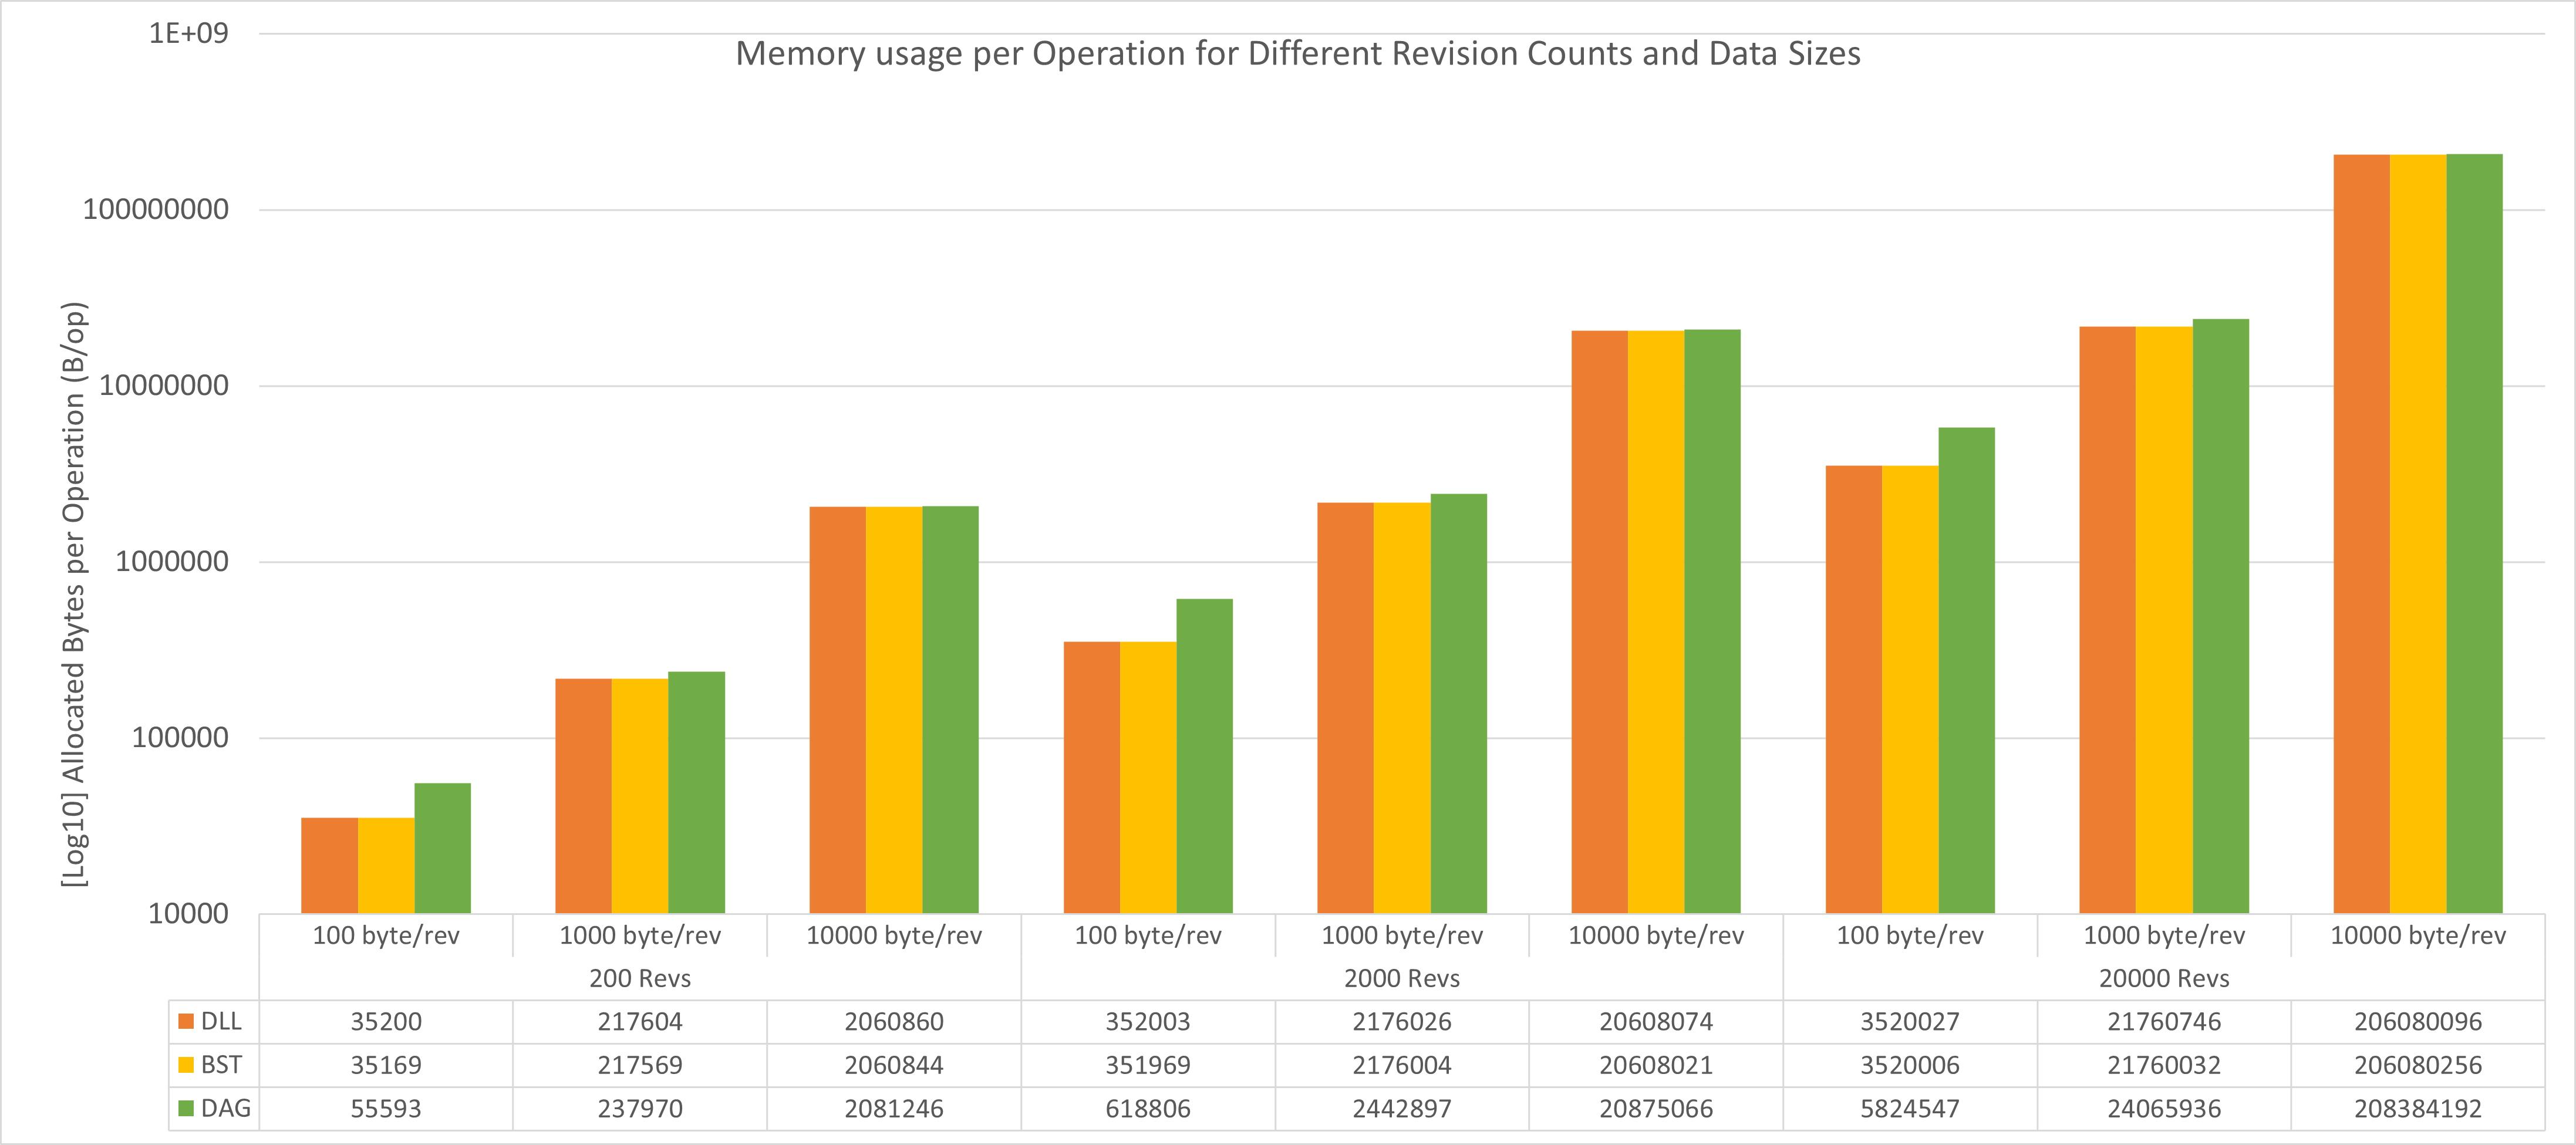
\includegraphics[width=1\linewidth]{charts/dataStruct_bytes_all.png}
        \caption{Memory Usage}
        \label{fig:data-structure-memory-usage}
    \end{subfigure}

    \begin{subfigure}[b]{0.75\textwidth}
        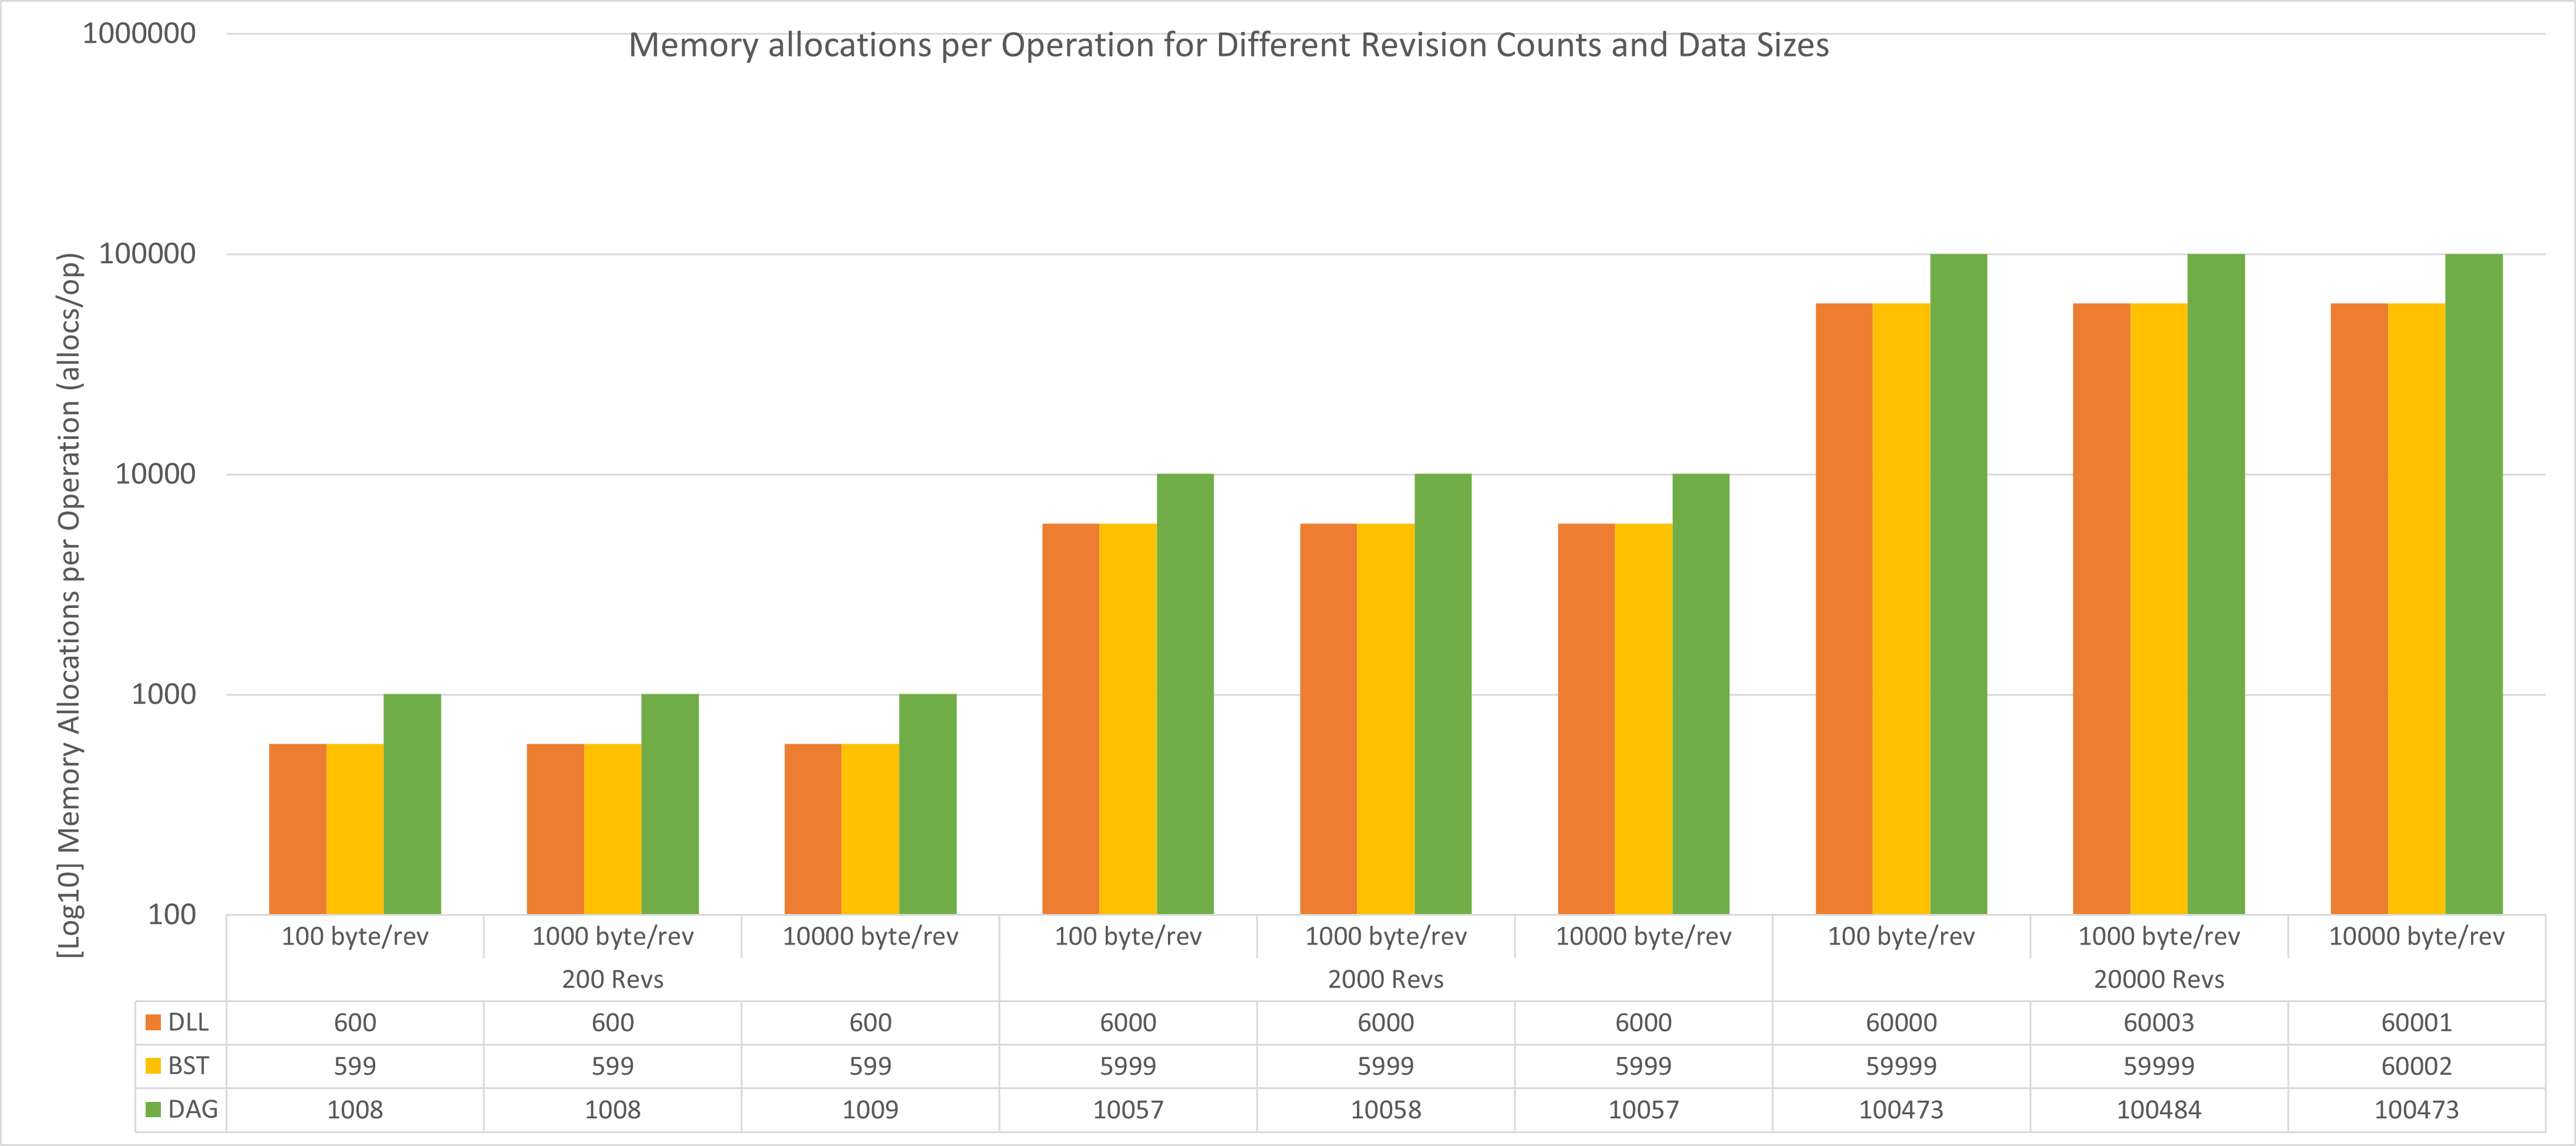
\includegraphics[width=1\linewidth]{charts/dataStruct_allocs_all.png}
        \caption{Memory Allocations}
        \label{fig:data-structure-memory-allocations}
    \end{subfigure}

    \caption{Performance metrics for all three Data Structure implementations.}
    \label{fig:data-structure-performance-metrics}
\end{figure}
\newpage

\paragraph{Execution Time}
Regarding execution time across the three data structures, we see that \lstinline{numRevisions} seems to have the most significant impact on the processing time, especially when the number of revisions is high. For a low and medium number of revisions, all three data structures have similar performance. However, once the number of revisions grows large enough, we start to see the \lstinline{Directed Acyclic Graph} handling small data sizes much better than the \lstinline{Doubly Linked List} and \lstinline{Binary Search Tree}.
\smallskip

\paragraph{Memory Usage}
The memory usage for the \lstinline{Doubly Linked List} and \lstinline{Binary Search Tree} appears to be relatively equal across all data sizes. However, the \lstinline{Directed Acyclic Graph} seems to require more memory at low and medium data sizes. This is likely due to the fact that the \lstinline{Directed Acyclic Graph} is storing the data in a map, which is a hash table. The \lstinline{Doubly Linked List} and \lstinline{Binary Search Tree} are storing the data in a slice, which is a contiguous block of memory.
\smallskip

\paragraph{Memory Allocations}
The memory allocation data mirrors the memory usage data, showing similar performance across the board for the \lstinline{Doubly Linked List} and \lstinline{Binary Search Tree} but higher memory requirements for the \lstinline{Directed Acyclic Graph}.

\section{Algorithms}

\subsection{Search Algorithms}

\begin{table}[h]
    \centering
    \begin{tabular}{|r|r|r|r|r|}
        \hline
        \multicolumn{1}{|c|}{\textbf{num\_revisions}} & \multicolumn{1}{c|}{\textbf{data\_size}} & \multicolumn{1}{c|}{\textbf{ns\_per\_op}} & \multicolumn{1}{c|}{\textbf{bytes\_per\_op}} & \multicolumn{1}{c|}{\textbf{allocs\_per\_op}} \\ \hline
        200 Revs                                      & 100 byte/rev                             & 192                                       & 0                                            & 0                                             \\ \hline
        200 Revs                                      & 1000 byte/rev                            & 191                                       & 0                                            & 0                                             \\ \hline
        200 Revs                                      & 10000 byte/rev                           & 190                                       & 0                                            & 0                                             \\ \hline
        2000 Revs                                     & 100 byte/rev                             & 1791                                      & 0                                            & 0                                             \\ \hline
        2000 Revs                                     & 1000 byte/rev                            & 1768                                      & 0                                            & 0                                             \\ \hline
        2000 Revs                                     & 10000 byte/rev                           & 1801                                      & 0                                            & 0                                             \\ \hline
        20000 Revs                                    & 100 byte/rev                             & 29180                                     & 0                                            & 0                                             \\ \hline
        20000 Revs                                    & 1000 byte/rev                            & 28773                                     & 0                                            & 0                                             \\ \hline
        20000 Revs                                    & 10000 byte/rev                           & 30309                                     & 0                                            & 0                                             \\ \hline
    \end{tabular}
    \caption{Performance metrics for the Linear Search algorithm.}
    \label{tab:linear-search-benchmark-results}
\end{table}
\smallskip

\begin{table}[h]
    \centering
    \begin{tabular}{|r|r|r|r|r|}
        \hline
        \multicolumn{1}{|c|}{\textbf{num\_revisions}} & \multicolumn{1}{c|}{\textbf{data\_size}} & \multicolumn{1}{c|}{\textbf{ns\_per\_op}} & \multicolumn{1}{c|}{\textbf{bytes\_per\_op}} & \multicolumn{1}{c|}{\textbf{allocs\_per\_op}} \\ \hline
        200 Revs                                      & 100 byte/rev                             & 360                                       & 0                                            & 0                                             \\ \hline
        200 Revs                                      & 1000 byte/rev                            & 360                                       & 0                                            & 0                                             \\ \hline
        200 Revs                                      & 10000 byte/rev                           & 357                                       & 0                                            & 0                                             \\ \hline
        2000 Revs                                     & 100 byte/rev                             & 3390                                      & 0                                            & 0                                             \\ \hline
        2000 Revs                                     & 1000 byte/rev                            & 3378                                      & 0                                            & 0                                             \\ \hline
        2000 Revs                                     & 10000 byte/rev                           & 3377                                      & 0                                            & 0                                             \\ \hline
        20000 Revs                                    & 100 byte/rev                             & 35875                                     & 0                                            & 0                                             \\ \hline
        20000 Revs                                    & 1000 byte/rev                            & 35717                                     & 0                                            & 0                                             \\ \hline
        20000 Revs                                    & 10000 byte/rev                           & 36296                                     & 0                                            & 0                                             \\ \hline
    \end{tabular}
    \caption{Performance metrics for the Binary Search algorithm.}
    \label{tab:binary-search-benchmark-results}
\end{table}

\begin{figure}[H]
    \centering
    \begin{subfigure}[b]{0.75\textwidth}
        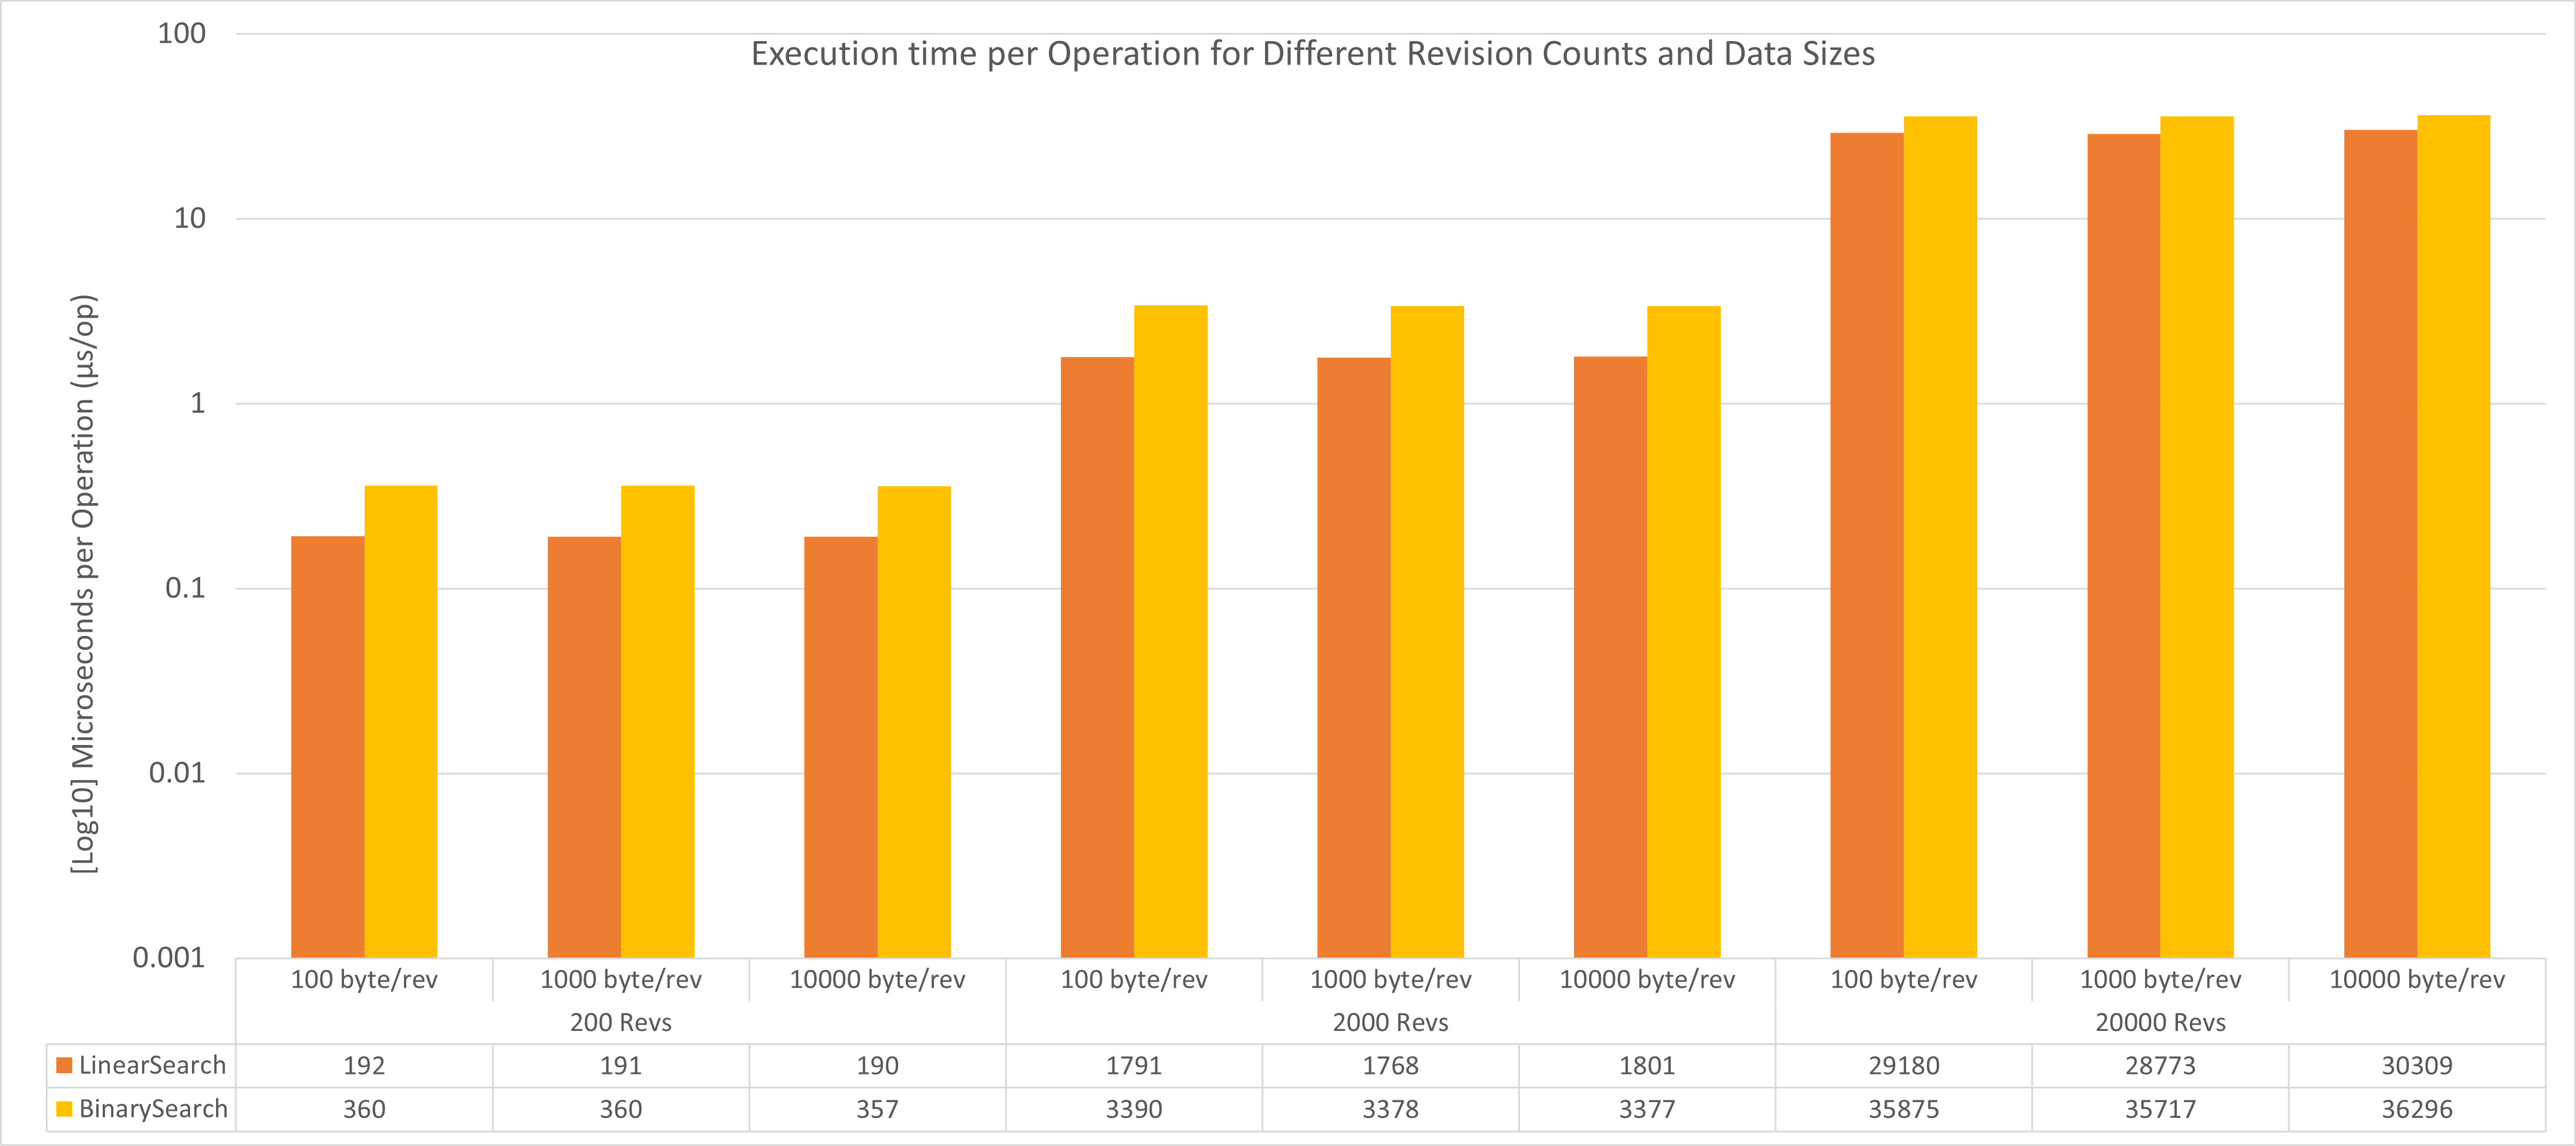
\includegraphics[width=1\linewidth]{charts/LS&BS_ns_all.png}
        \caption{Execution Time}
        \label{fig:linear-search-binary-search-execution-time}
    \end{subfigure}

    \caption{Execution time for the Linear Search and Binary Search algorithms.}
    \label{fig:linear-search-binary-search-performance-metrics}
\end{figure}

\paragraph{Execution Time}
The execution time for the \lstinline{Linear Search} and \lstinline{Binary Search} algorithms is very similar across all data sizes. This is likely due to the fact that the \lstinline{Linear Search} algorithm is iterating through the entire data set, regardless of the data size. The \lstinline{Binary Search} algorithm is also iterating through the entire data set, but it is doing so in a more efficient manner. The \lstinline{Binary Search} algorithm is able to skip over half of the data set with each iteration, therefore it should prove to be more efficient than the \lstinline{Linear Search} algorithm, so it is unclear why the execution time is so similar or even worse in some cases.

\paragraph{Memory Usage}
The \lstinline{Linear Search} and \lstinline{Binary Search} algorithms both have a memory usage of 0 bytes per operation. This is because the algorithms are not allocating any memory during their execution.

\paragraph{Memory Allocation}
The \lstinline{Linear Search} and \lstinline{Binary Search} algorithms both have a memory allocation of 0 allocations per operation. This is because the algorithms are not allocating any memory during their execution.

\newpage

\begin{table}[H]
    \centering
    \begin{tabular}{|r|r|r|r|r|}
        \hline
        \multicolumn{1}{|c|}{\textbf{num\_revisions}} & \multicolumn{1}{c|}{\textbf{data\_size}} & \multicolumn{1}{c|}{\textbf{ns\_per\_op}} & \multicolumn{1}{c|}{\textbf{bytes\_per\_op}} & \multicolumn{1}{c|}{\textbf{allocs\_per\_op}} \\ \hline
        200 Revs                                      & 100 byte/rev                             & 8670                                      & 4248                                         & 15                                            \\ \hline
        200 Revs                                      & 1000 byte/rev                            & 8698                                      & 4264                                         & 15                                            \\ \hline
        200 Revs                                      & 10000 byte/rev                           & 8863                                      & 4259                                         & 15                                            \\ \hline
        2000 Revs                                     & 100 byte/rev                             & 91438                                     & 47907                                        & 68                                            \\ \hline
        2000 Revs                                     & 1000 byte/rev                            & 93066                                     & 47916                                        & 68                                            \\ \hline
        2000 Revs                                     & 10000 byte/rev                           & 85277                                     & 47833                                        & 68                                            \\ \hline
        20000 Revs                                    & 100 byte/rev                             & 1092353                                   & 474162                                       & 360                                           \\ \hline
        20000 Revs                                    & 1000 byte/rev                            & 886706                                    & 475409                                       & 361                                           \\ \hline
        20000 Revs                                    & 10000 byte/rev                           & 839202                                    & 476277                                       & 361                                           \\ \hline
    \end{tabular}
    \caption{Performance metrics for the Depth First Search algorithm.}
    \label{tab:depth-first-search-benchmark-results}
\end{table}
\begin{table}[h]
    \centering
    \begin{tabular}{|r|r|r|r|r|}
        \hline
        \multicolumn{1}{|c|}{\textbf{num\_revisions}} & \multicolumn{1}{c|}{\textbf{data\_size}} & \multicolumn{1}{c|}{\textbf{ns\_per\_op}} & \multicolumn{1}{c|}{\textbf{bytes\_per\_op}} & \multicolumn{1}{c|}{\textbf{allocs\_per\_op}} \\ \hline
        200 Revs                                      & 100 byte/rev                             & 14648                                     & 5044                                         & 114                                           \\ \hline
        200 Revs                                      & 1000 byte/rev                            & 14538                                     & 5052                                         & 115                                           \\ \hline
        200 Revs                                      & 10000 byte/rev                           & 14817                                     & 5058                                         & 115                                           \\ \hline
        2000 Revs                                     & 100 byte/rev                             & 146733                                    & 55869                                        & 1066                                          \\ \hline
        2000 Revs                                     & 1000 byte/rev                            & 148890                                    & 55971                                        & 1067                                          \\ \hline
        2000 Revs                                     & 10000 byte/rev                           & 141562                                    & 55981                                        & 1068                                          \\ \hline
        20000 Revs                                    & 100 byte/rev                             & 1479317                                   & 561308                                       & 10478                                         \\ \hline
        20000 Revs                                    & 1000 byte/rev                            & 1405637                                   & 550430                                       & 10323                                         \\ \hline
        20000 Revs                                    & 10000 byte/rev                           & 1394722                                   & 556945                                       & 10399                                         \\ \hline
    \end{tabular}
    \caption{Performance metrics for the Breadth First Search algorithm.}
    \label{tab:breadth-first-search-benchmark-results}
\end{table}
% \newpage

\begin{figure}[H]
    \centering
    \begin{subfigure}[b]{0.75\textwidth}
        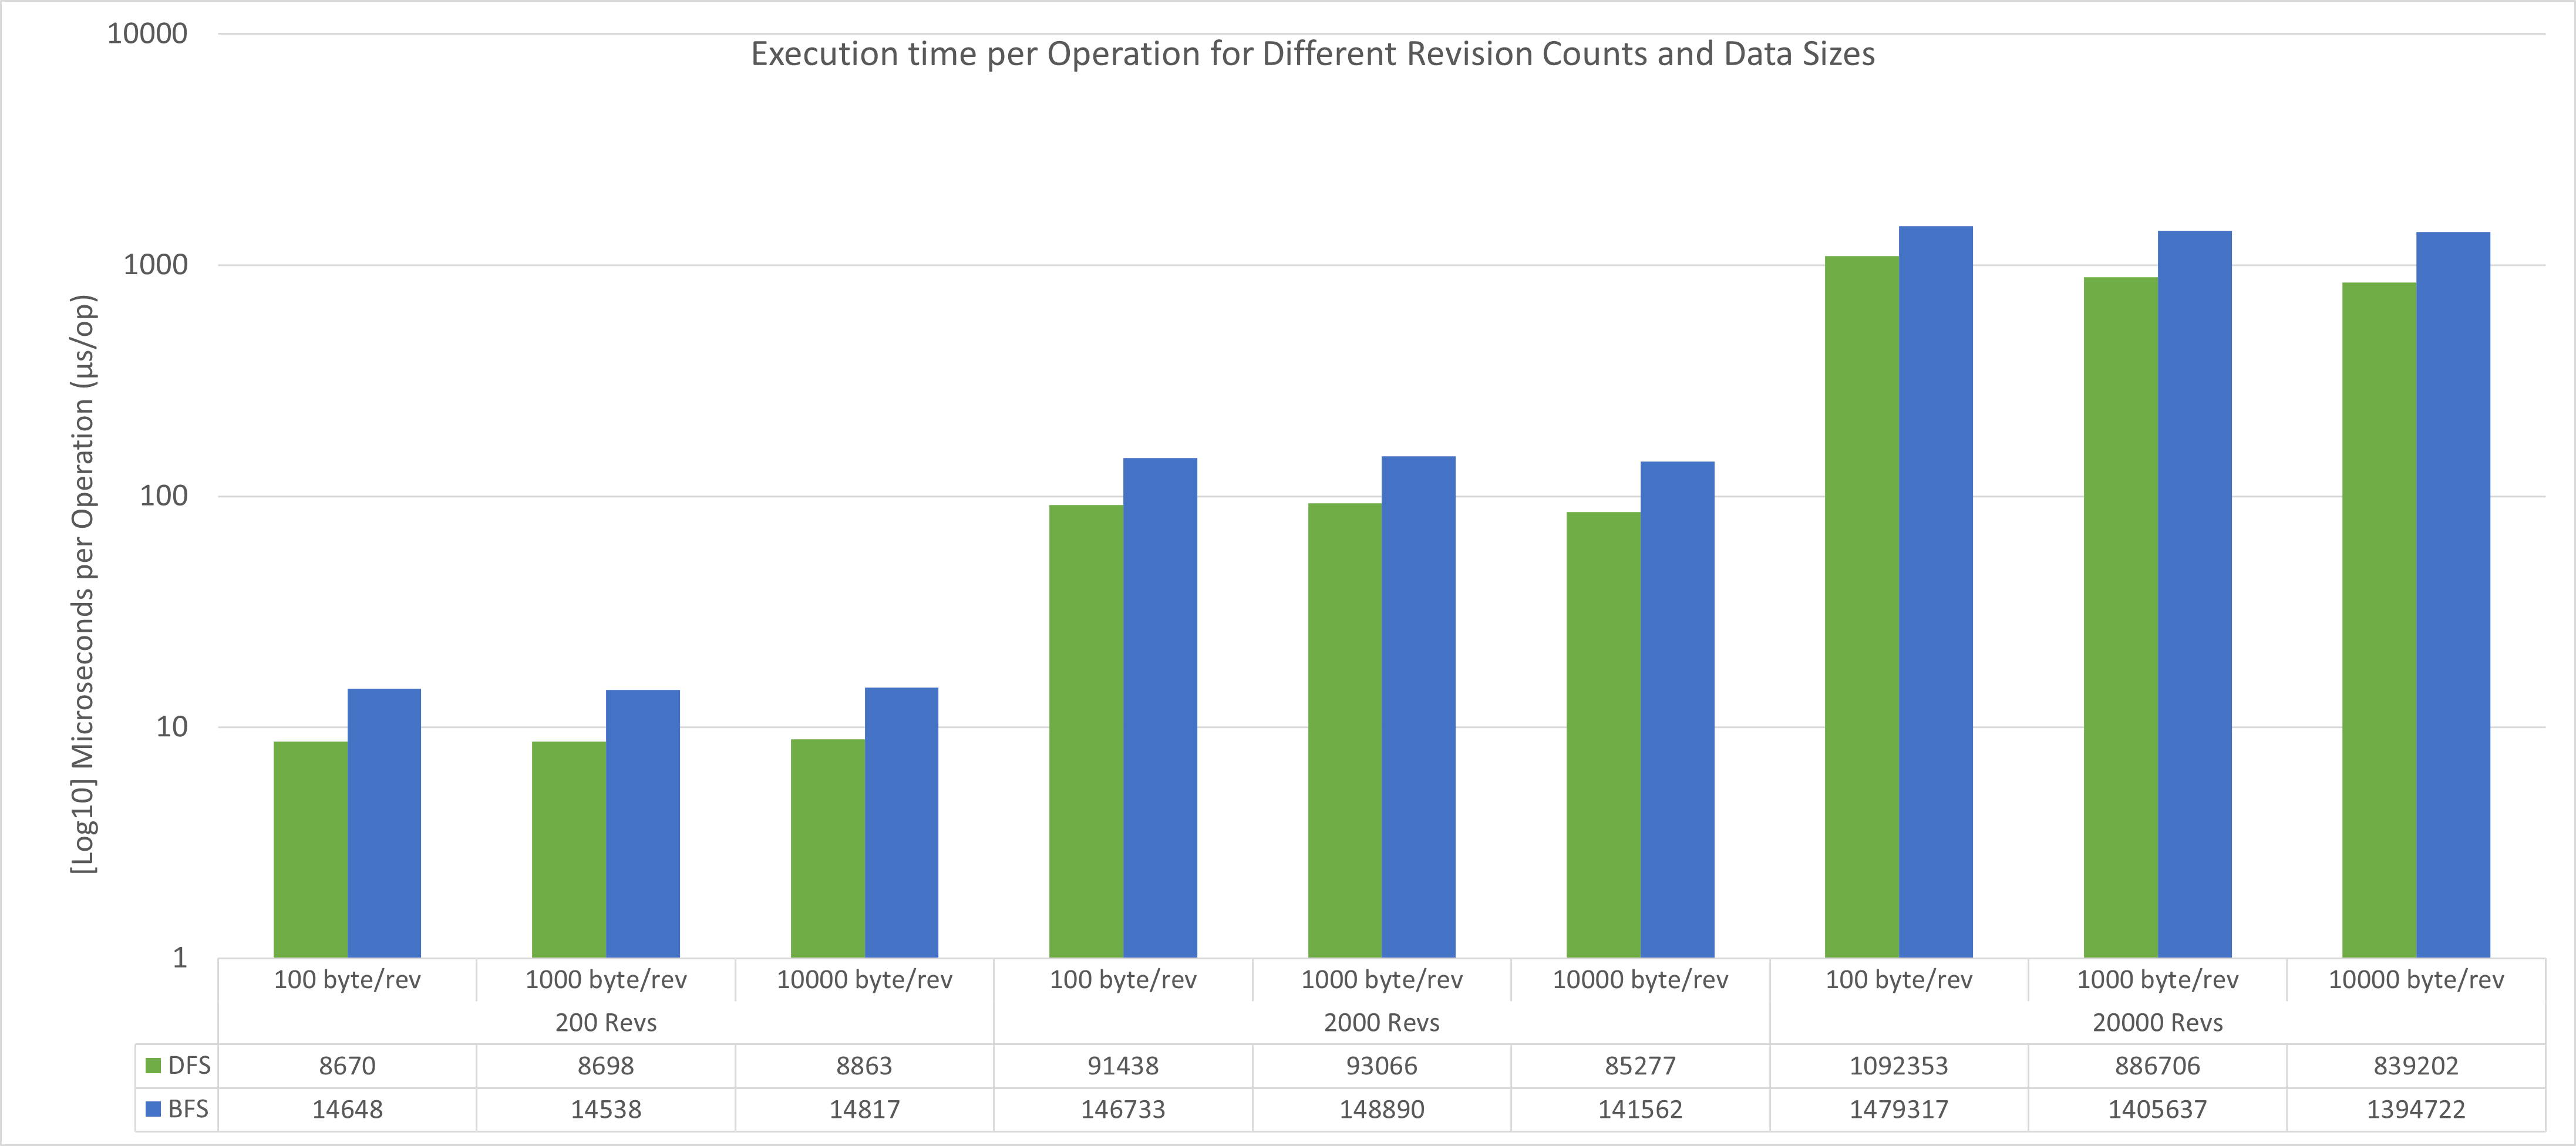
\includegraphics[width=1\linewidth]{charts/DFS&BFS_ns_all.png}
        \caption{Execution Time}
        \label{fig:depth-first-search-breadth-first-search-execution-time}
    \end{subfigure}

    \begin{subfigure}[b]{0.75\textwidth}
        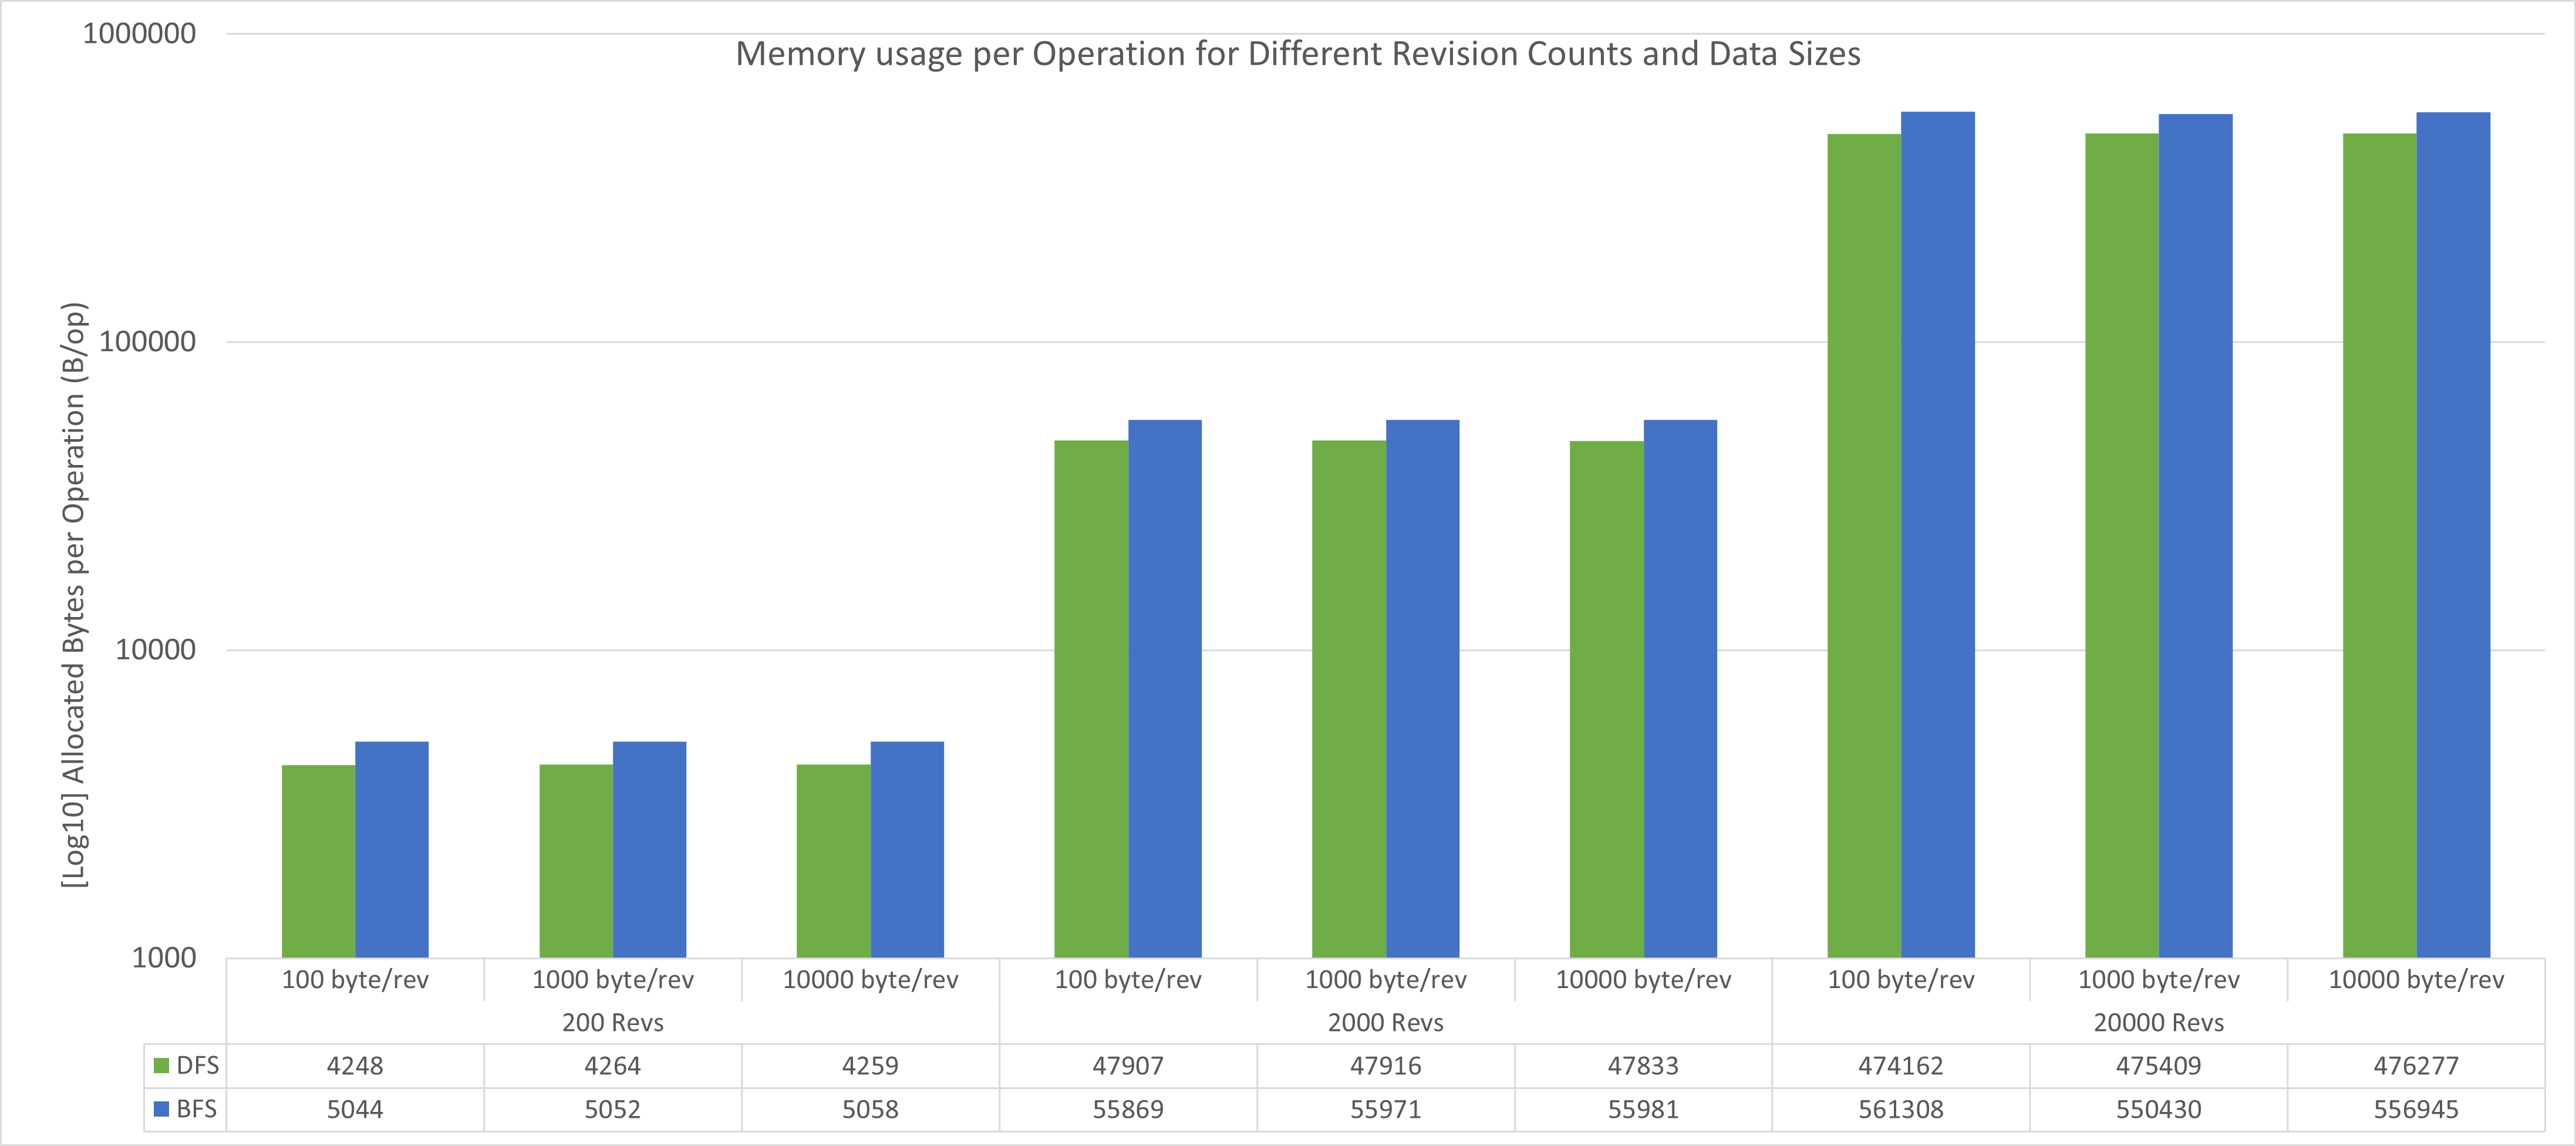
\includegraphics[width=1\linewidth]{charts/DFS&BFS_bytes_all.png}
        \caption{Memory Usage}
        \label{fig:depth-first-search-breadth-first-search-memory-usage}
    \end{subfigure}

    \begin{subfigure}[b]{0.75\textwidth}
        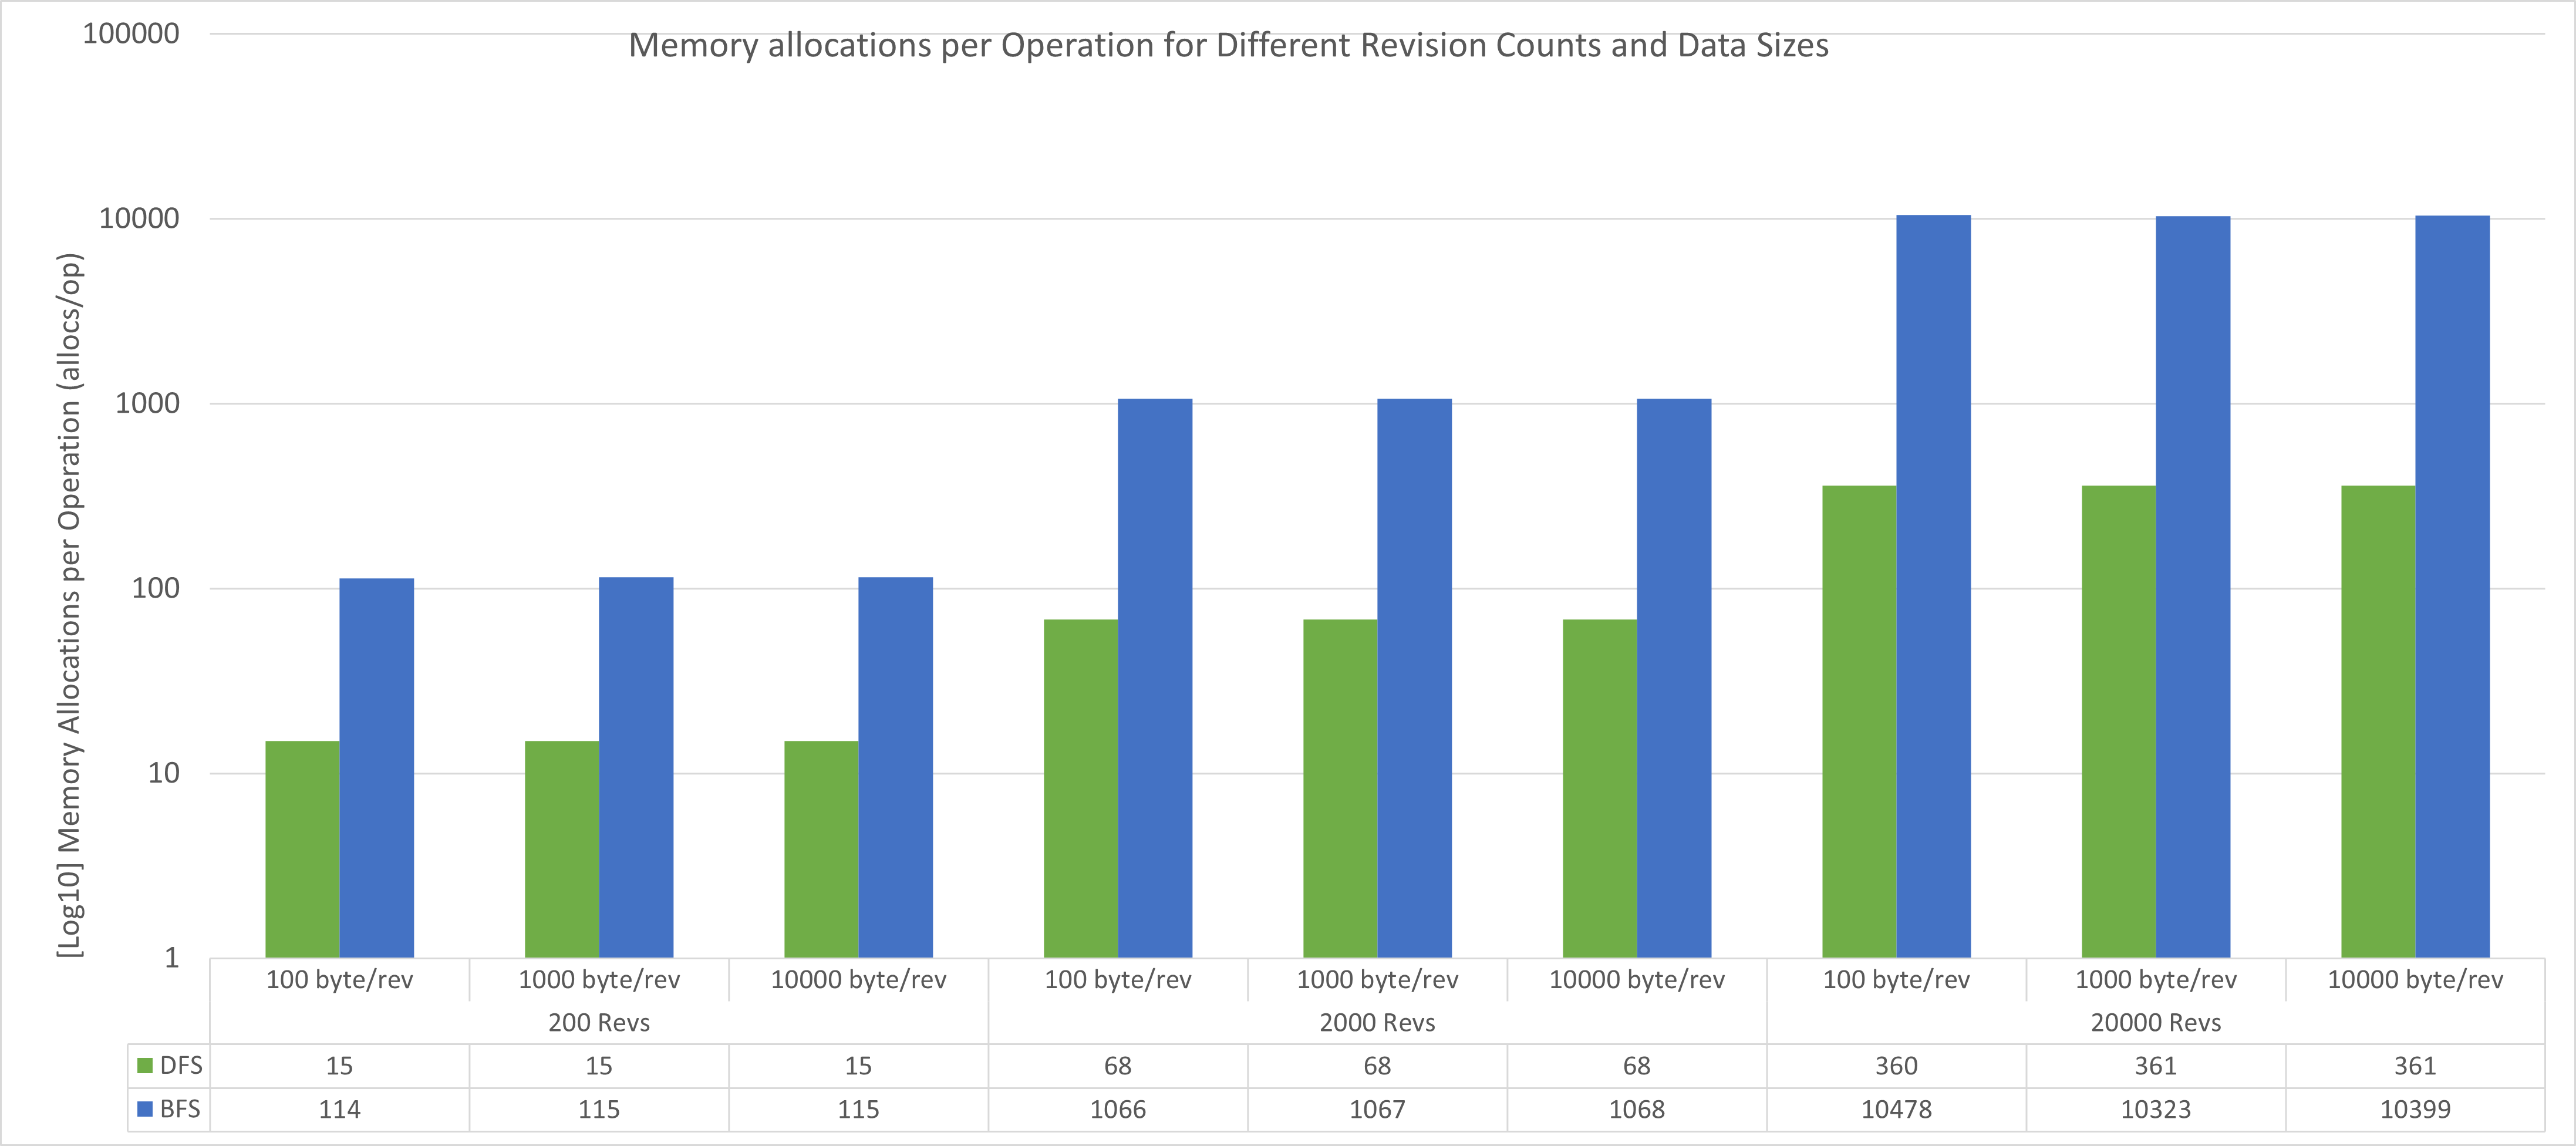
\includegraphics[width=1\linewidth]{charts/DFS&BFS_allocs_all.png}
        \caption{Memory Allocations}
        \label{fig:depth-first-search-breadth-first-search-memory-allocations}
    \end{subfigure}

    \caption{Performance metrics for the Depth First Search and Breadth First Search algorithms.}
    \label{fig:depth-first-search-breadth-first-search-performance-metrics}
\end{figure}

\paragraph{Execution Time}
The execution time gap between the \lstinline{Depth First Search} and \lstinline{Breadth First Search} algorithms stays relatively similar as the number of revisions increases. The \lstinline{Depth First Search} algorithm is consistently faster than the \lstinline{Breadth First Search} algorithm.

\paragraph{Memory Usage}
The memory usage gap between the \lstinline{Depth First Search} and \lstinline{Breadth First Search} algorithms stays relatively similar as the number of revisions increases. The \lstinline{Depth First Search} algorithm consistently uses less memory than the \lstinline{Breadth First Search} algorithm.

\paragraph{Memory Allocations}
The memory allocation gap between the \lstinline{Depth First Search} and \lstinline{Breadth First Search} algorithms is much wider than the execution time and memory usage gaps. The \lstinline{Depth First Search} algorithm consistently allocates much less memory than the \lstinline{Breadth First Search} algorithm.

\newpage

\subsection{Diff Algorithms}

\begin{table}[h]
    \centering
    \begin{tabular}{|l|r|r|r|}
        \hline
        \multicolumn{1}{|c|}{\textbf{test\_case}} & \multicolumn{1}{c|}{\textbf{ns\_per\_op}} & \multicolumn{1}{c|}{\textbf{bytes\_per\_op}} & \multicolumn{1}{c|}{\textbf{allocs\_per\_op}} \\ \hline
        Small                                     & 2231                                      & 2008                                         & 36                                            \\ \hline
        Large                                     & 161544303                                 & 74748939                                     & 22243                                         \\ \hline
        Extreme                                   & 159264376                                 & 74717878                                     & 21757                                         \\ \hline
    \end{tabular}
    \caption{Performance metrics for the Myers Diff algorithm.}
    \label{tab:myers-diff-benchmark-results}
\end{table}
\begin{table}[h]
    \centering
    \begin{tabular}{|l|r|r|r|}
        \hline
        \multicolumn{1}{|c|}{\textbf{test\_case}} & \multicolumn{1}{c|}{\textbf{ns\_per\_op}} & \multicolumn{1}{c|}{\textbf{bytes\_per\_op}} & \multicolumn{1}{c|}{\textbf{allocs\_per\_op}} \\ \hline
        Small                                     & 3987                                      & 3081                                         & 64                                            \\ \hline
        Large                                     & 344500                                    & 378884                                       & 6071                                          \\ \hline
        Extreme                                   & 123503                                    & 204634                                       & 2047                                          \\ \hline
    \end{tabular}
    \caption{Performance metrics for the Patience Diff algorithm.}
    \label{tab:patience-diff-benchmark-results}
\end{table}

\begin{figure}[h]
    \centering
    \begin{subfigure}[b]{0.75\textwidth}
        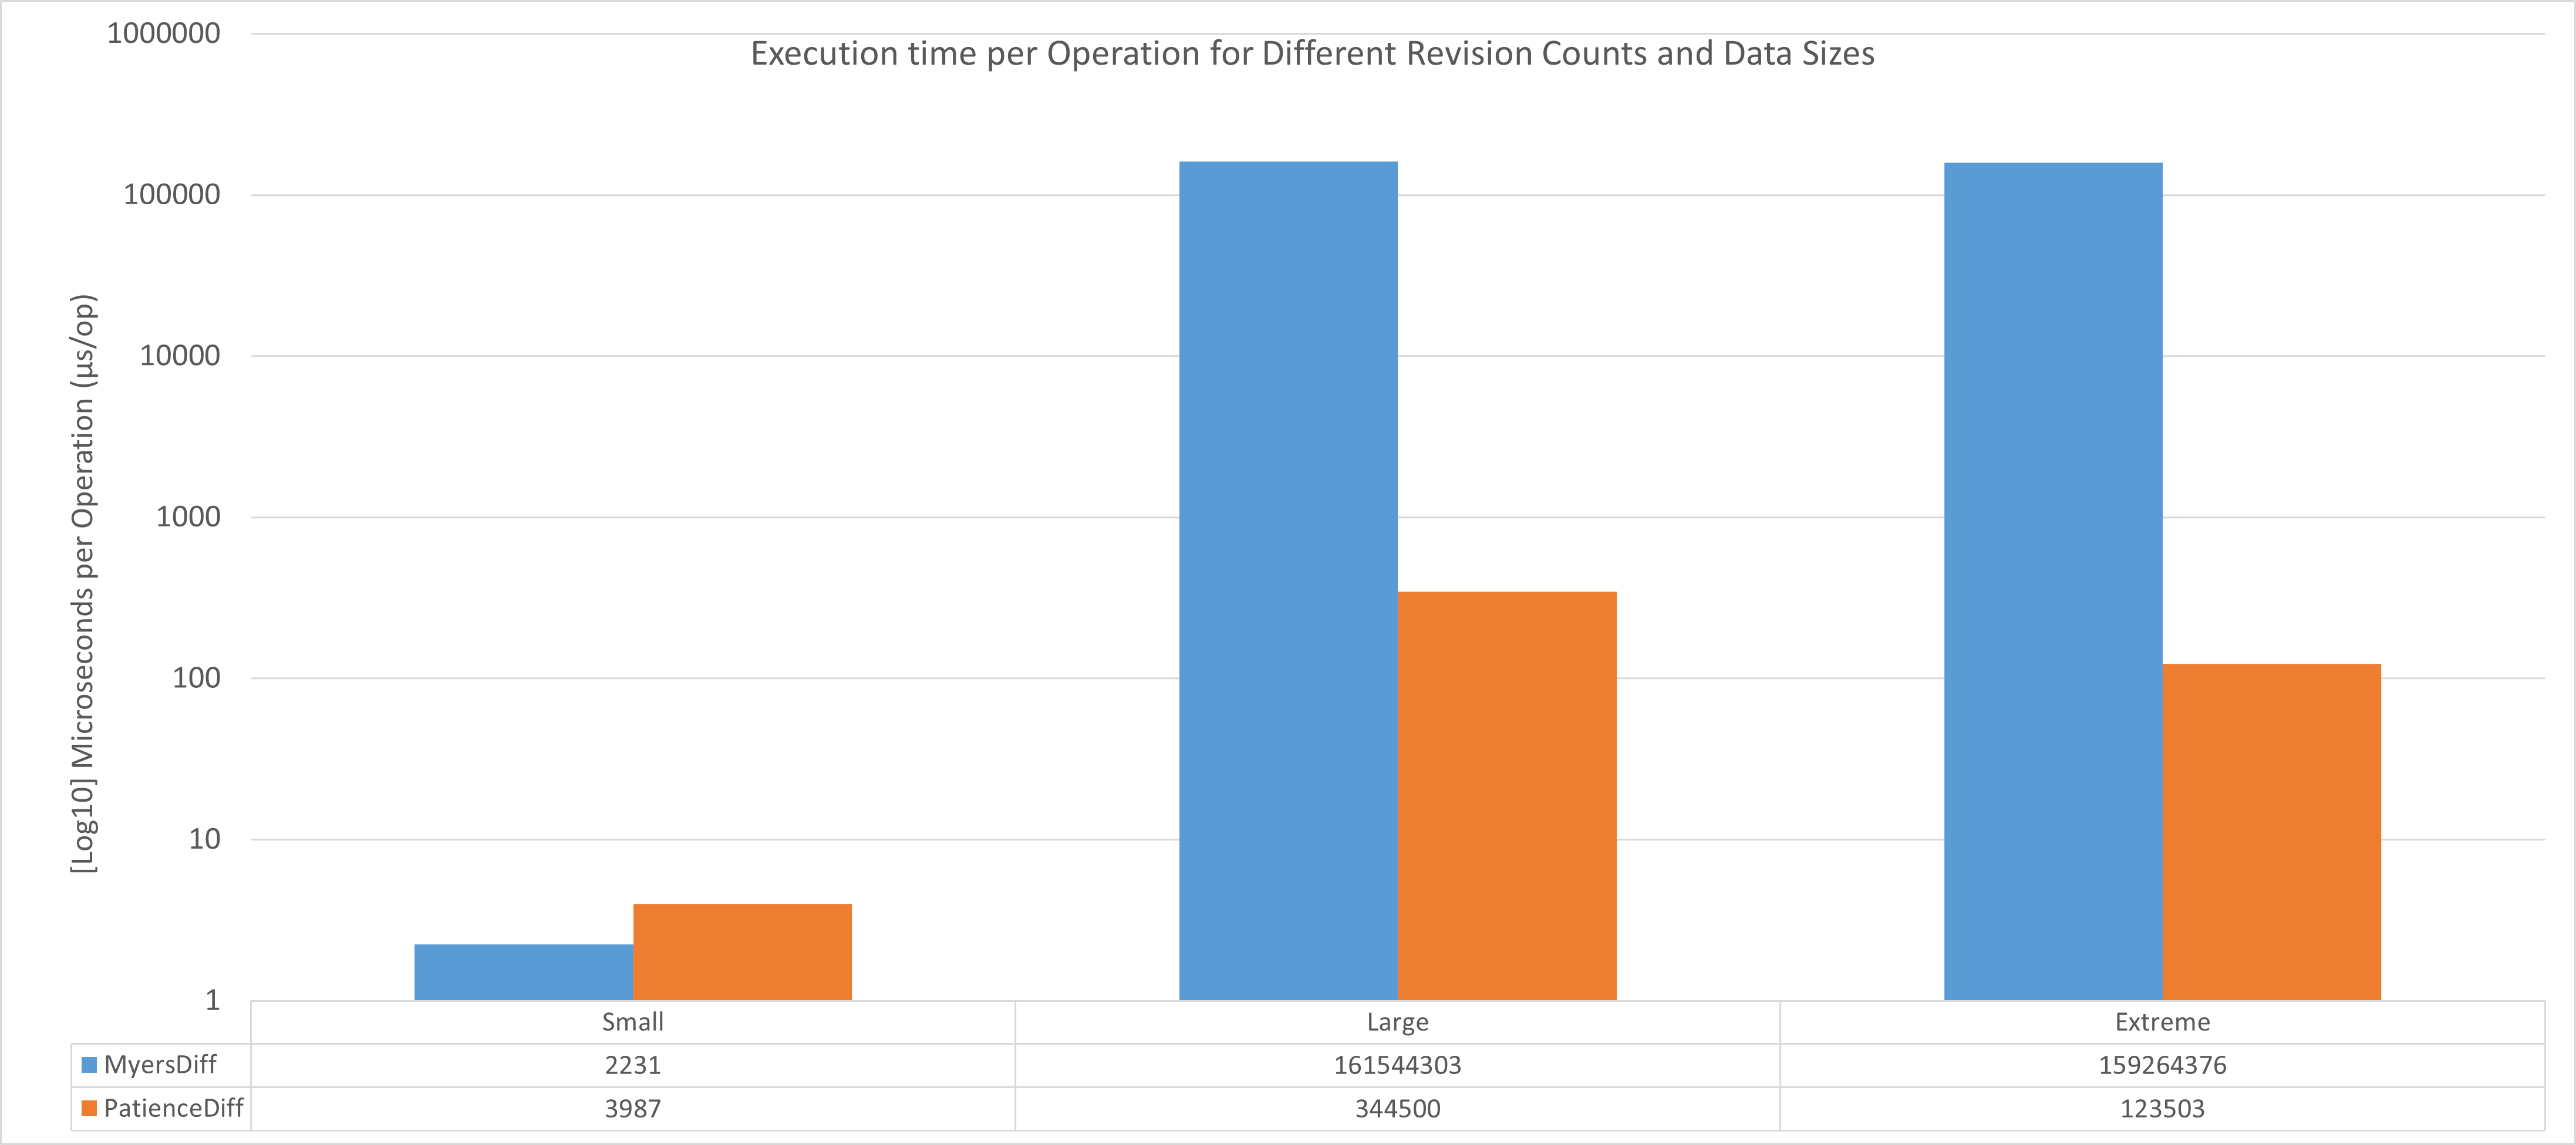
\includegraphics[width=1\linewidth]{charts/diff_ns_all.png}
        \caption{Execution Time}
        \label{fig:myers-diff-patience-diff-execution-time}
    \end{subfigure}

    \begin{subfigure}[b]{0.75\textwidth}
        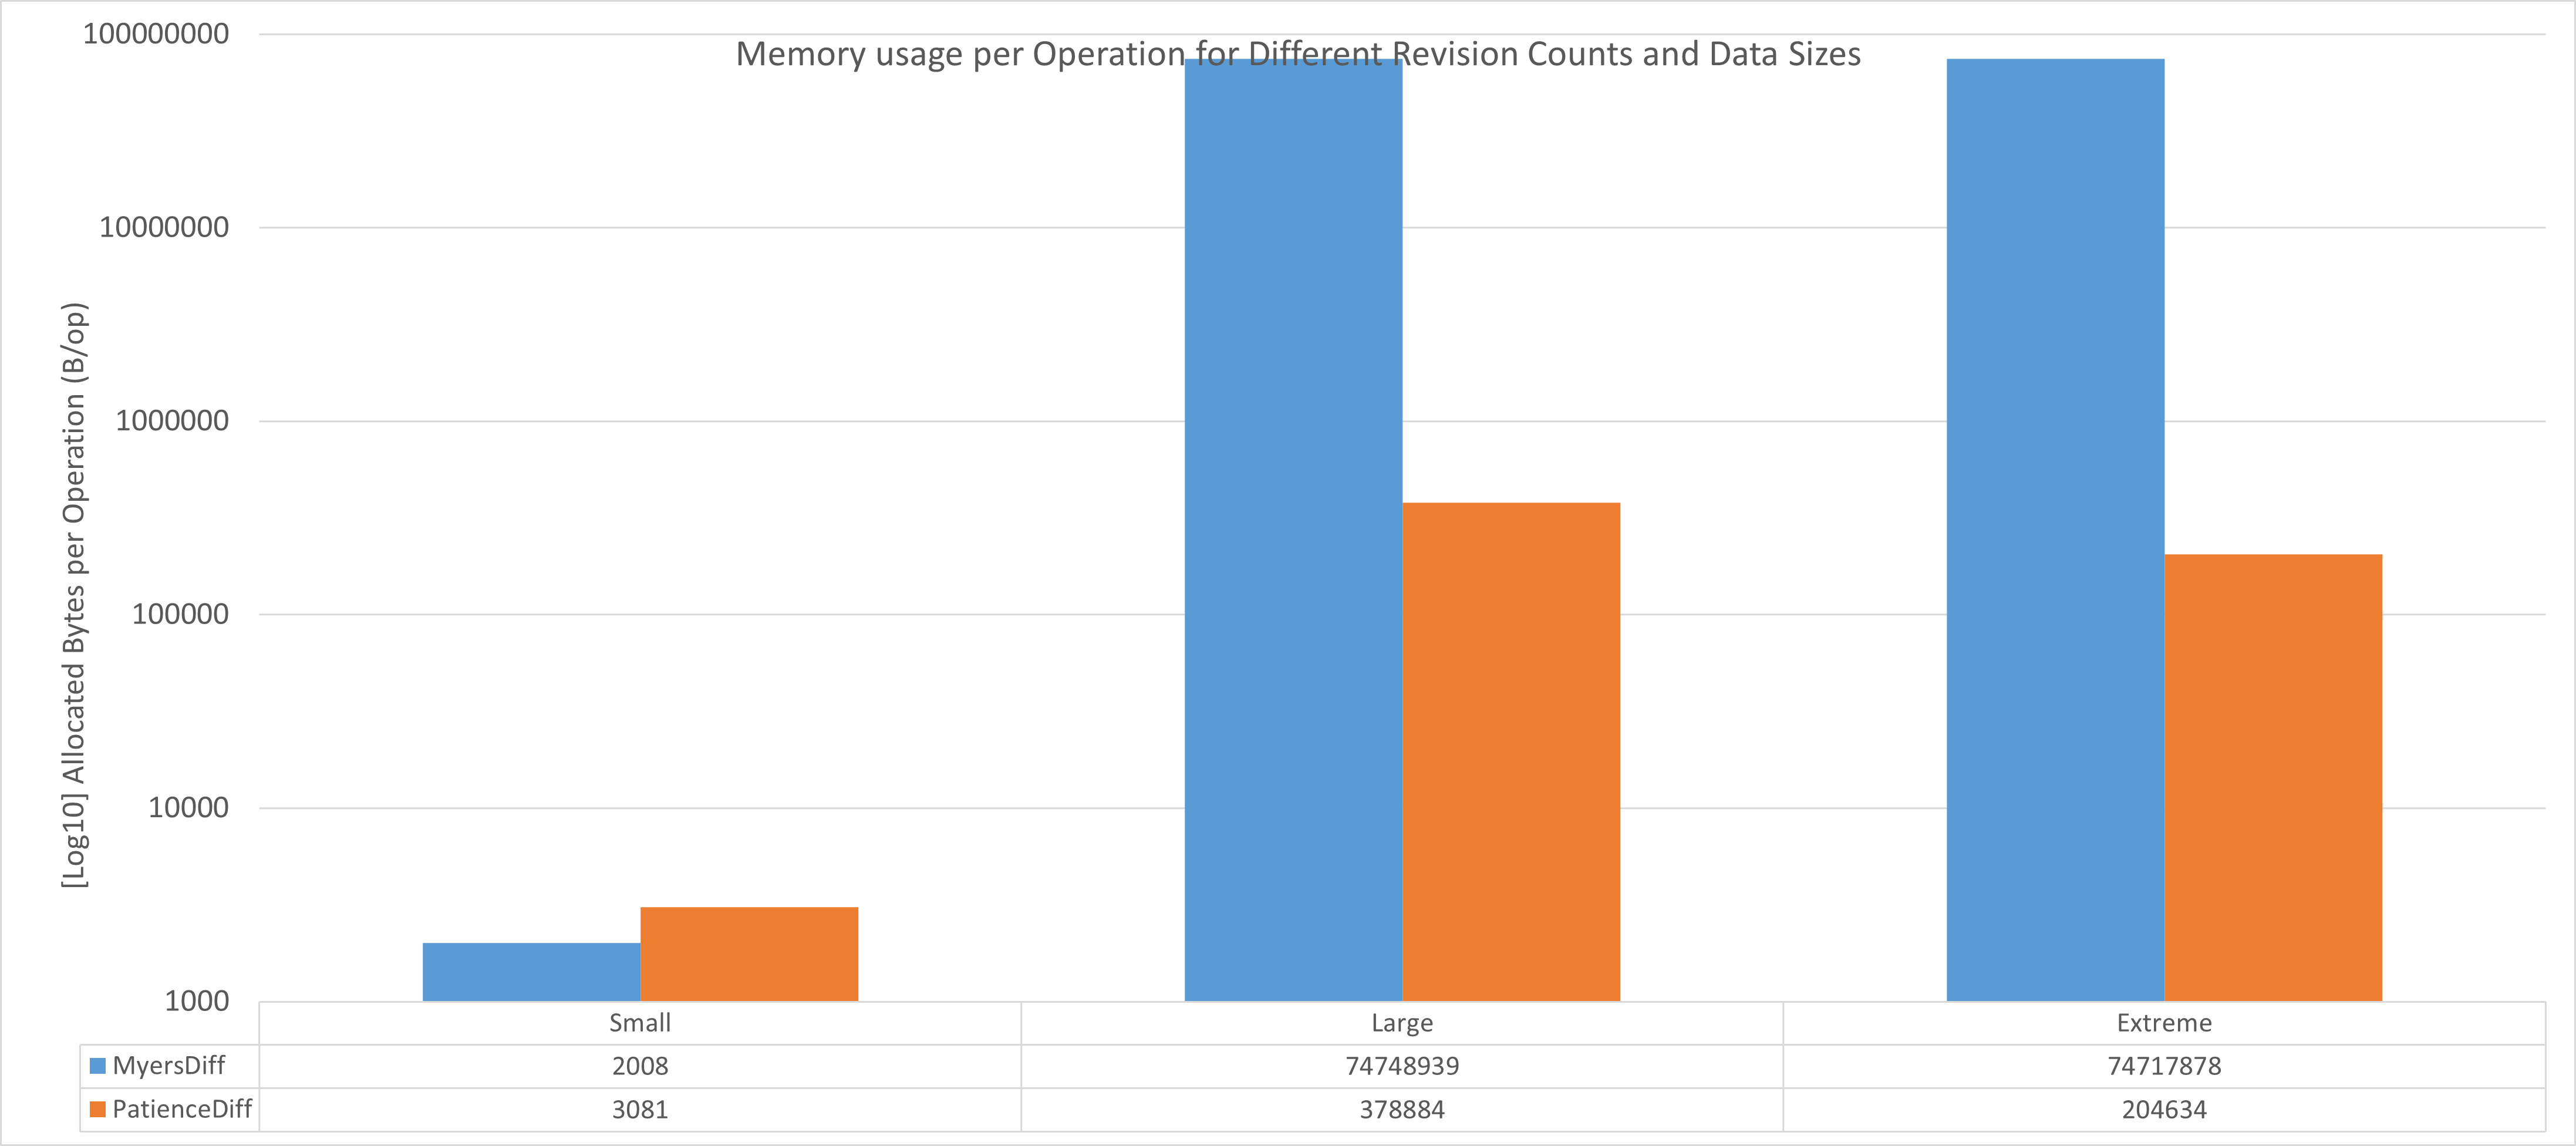
\includegraphics[width=1\linewidth]{charts/diff_bytes_all.png}
        \caption{Memory Usage}
        \label{fig:myers-diff-patience-diff-memory-usage}
    \end{subfigure}

    \begin{subfigure}[b]{0.75\textwidth}
        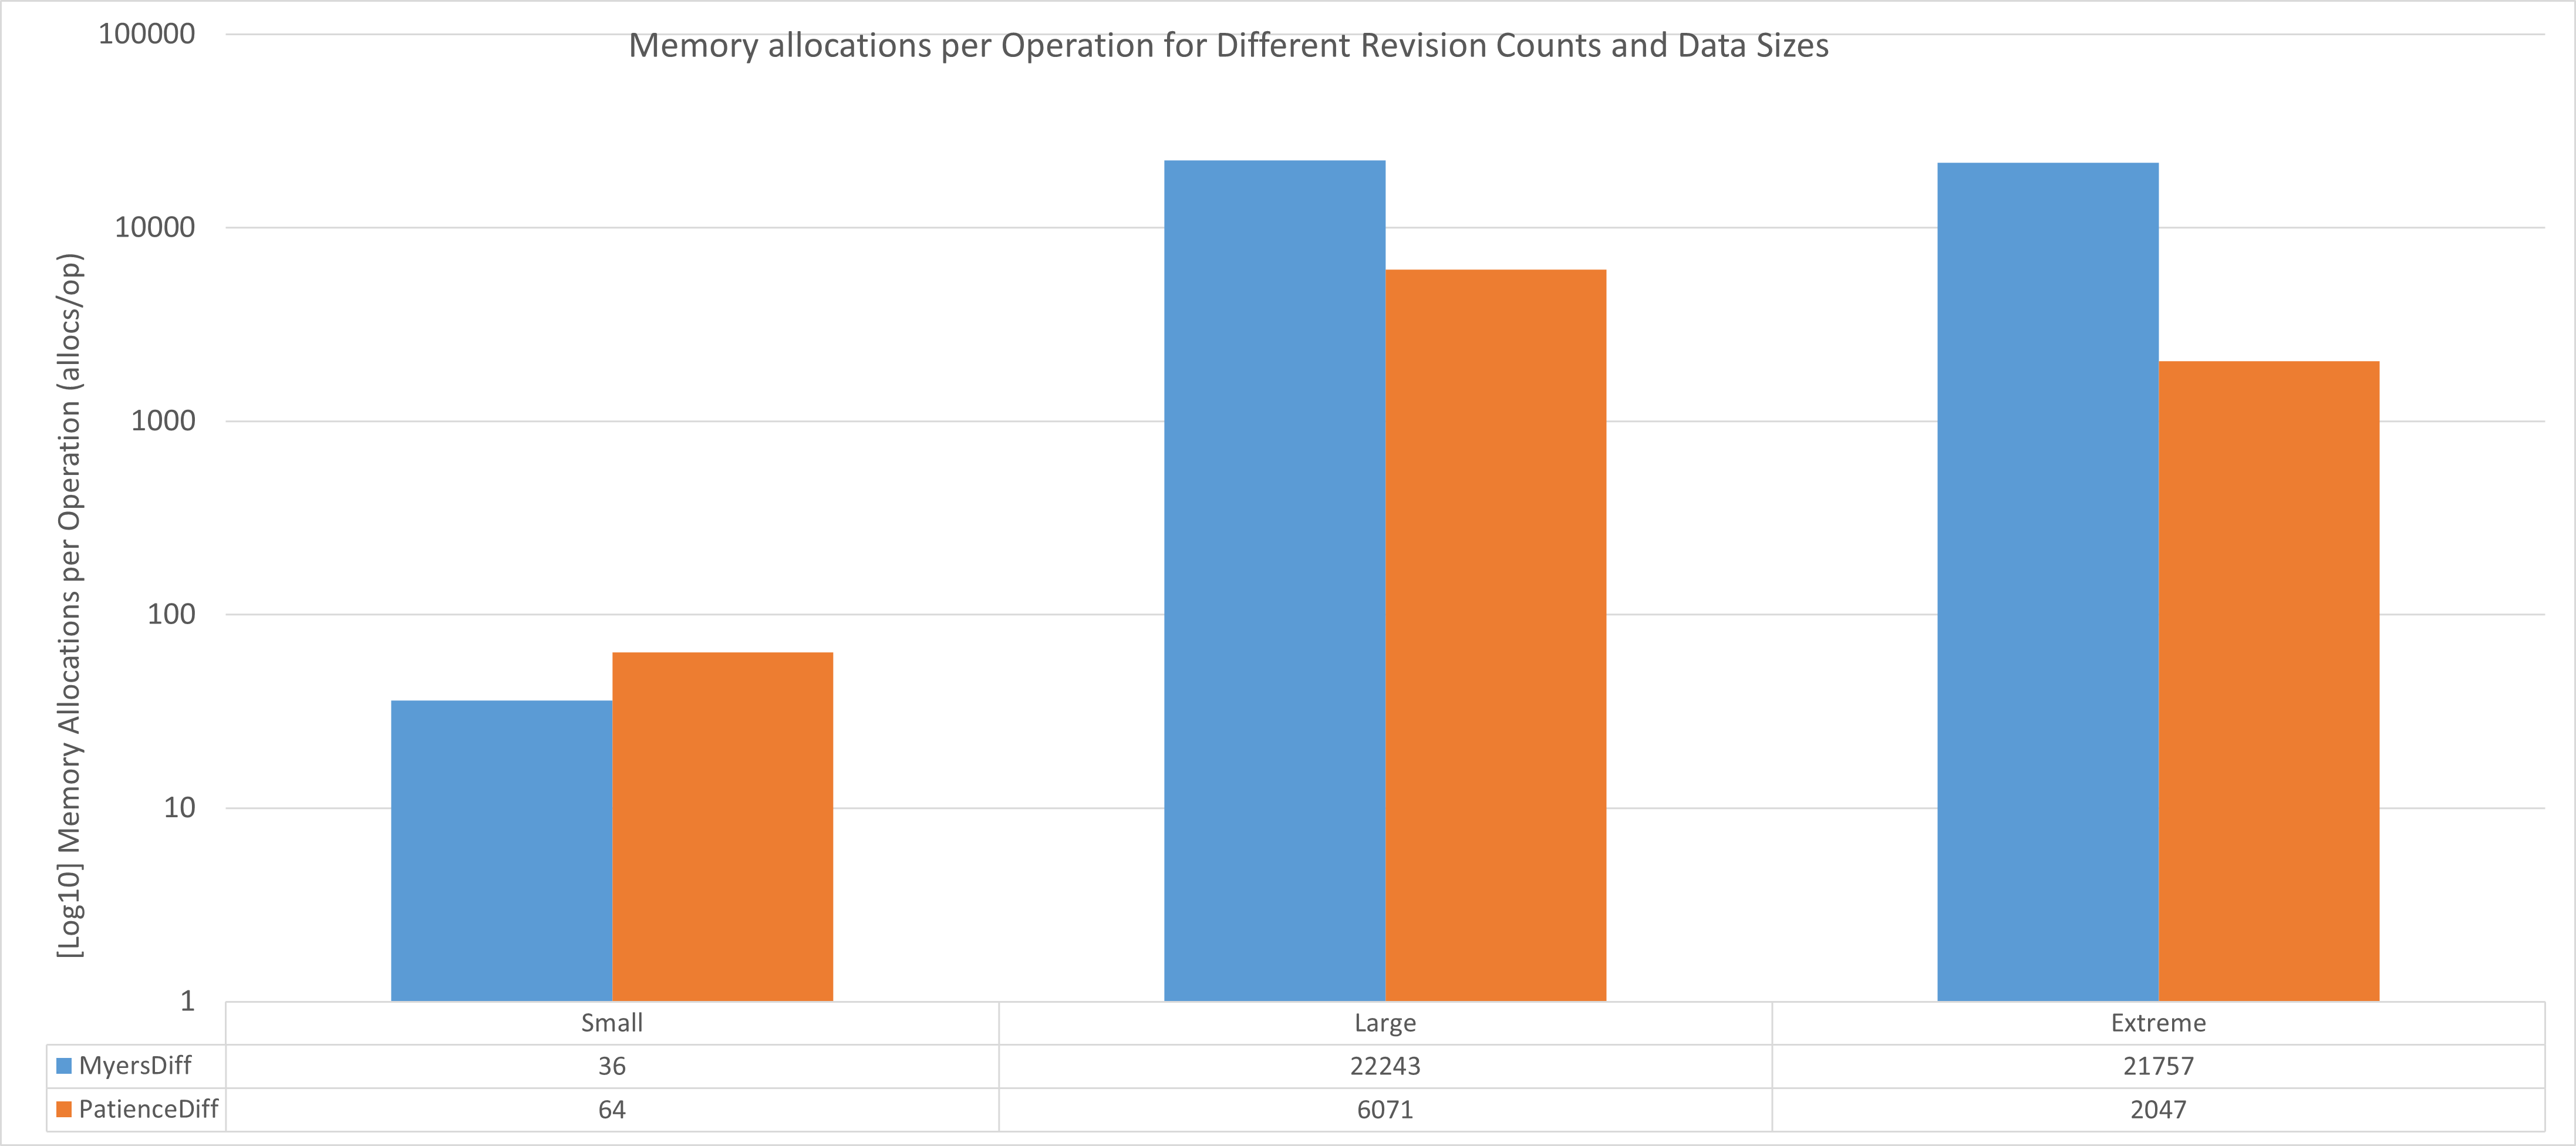
\includegraphics[width=1\linewidth]{charts/diff_allocs_all.png}
        \caption{Memory Allocations}
        \label{fig:myers-diff-patience-diff-memory-allocations}
    \end{subfigure}

    \caption{Performance metrics for the Myers Diff and Patience Diff algorithms.}
    \label{fig:myers-diff-patience-diff-performance-metrics}
\end{figure}

